\chapter{Methods and Implementation}\label{cha:Method}

% längsta avsnittet i rapporten. Den består av en redogörelse av ditt arbete och den visar hur du kommer fram till dina resultat.

% Undvik egna synpunkter. Dessa framförs i Inledningskapitlet och Diskussions-kapitlet

% Ange källa till figurer i slutet. T.ex.  Source: Expedition Mondial.

% Metoddelen beskriver tillvägagångssättet – intervjuer, observationer, litteraturstudier, laborationer och så vidare. Motivera varför en viss metod valdes och vilka eventuella svårigheter som har förekommit. Metoden ska vara replikerbar, vilket innebär att en annan skribent ska kunna göra om studien med hjälp av informationen i metoddelen. Det finns en mängd böcker om olika vetenskapliga metoder. Till exempel kan en intervju utföras på en mängd olika sätt. I rapporter inom humaniora brukar metoddelen vara mer utförlig än i en teknisk rapport.

This chapter presents the methodological framework, via presenting methods to design for learning and motivation.

Then, the setting and research context is described, together with a description of the participants.

Then, application implementation is described, followed by presenting the study design and data collection.

The final topic is data analysis theory.

\section{Methodological framework}

\subsection{Design for Learning}

%\citepp{effectivelearning-robert}
%\citepp{learning-krathwohl}
%\citepp{learning-ucla}

The following sections, are about how to design for effective learning \citep{dirksen}, by designing for the mind, cognitive psychology. % Design for How People Learn (book, torrent)

Cognitive psychology deals with how our brain works in regards to our memory.

The section presents strategies and techniques to design learning for the mind, and what needs to be considered.

Two aspects are especially relevant when it comes to education: how humans can be supported to retaining (the first section) and retrieving (the second section) communicated information.

In how humans learn, the purpose is to find the most powerful strategies and techniques to design effective learning (mapping educational objectives, how to build skills, pattern-matching techniques, and the power of reflection and assessing).

In how people forget, UCLA Bjork's Learning and Forgetting Lab \citep{bjork} researches how people forget, and how to design so that people do not forget ( retrieval practice and spaced practice).

%On January 28th, 2016, Henrik Marklund\ref{effectivelearning-expert} at the educautional technology startup Knowly was interviewed about Pedagogic Development. He means there are two main areas of research, and an additional one.
%The third area, training transfer, is the research on how to make sure a course gives effect in everyday life.

%The third area is training transfer, and asks "How do you make sure a course gives effect in your everyday life?". For YoungDrive, the wish is that the coach training gives effect in the coaches' everyday life. The master thesis aims to be able to assess and encourage this.

%\subsection{Pedagogical development}

%The first section describes "How do you get people to learn things?", cognitive psychology. Often school is studied, where learning is about being taught a subject, and then to pass a test. E-learning tools are often designed to do similar things to what schools does.

%The second section describes "How do you get people to behave differently?", social psychology. One area of research is about building habits. This is highly relevant in e-learning, where behavior change may be necessary to build the habit of using an app or a digital tool repeatedly.

%\include{theory/learning/pedagogical-development/cognitive_psychology}

%\subsubsubsection{Learning}

  \subsubsection{Learning Entrepreneurship: Mapping Educational Objectives with Bloom's Revised Taxonomy}

  What to teach should be determined by the learning objectives of the activity.

  Learning activities often involve both lower order and higher order thinking skills as well as a mix of concrete and abstract knowledge. This needs to be designed for. Here, Bloom's revised taxonomy can provide usable insight into how to design, by the combination between lower or higher cognitive complexity, and concrete (factual or conceptual) or abstract knowledge (procedural or metacognitive). \cite{cheong} The taxonomy thus provides a framework for determining and clarifying learning objectives. See figure \ref{fig:revised-bloom} from \cite{heer}. Each colored block is an example of a learning objective matching with the two dimensions. The figure also explains the different concepts. Depending on the objective, it fits differently into the Knowledge dimension and Cognitive Process dimension of Bloom's Revised Taxonomy. \cite{bloom}

  \begin{figure}[h]
    \centering
    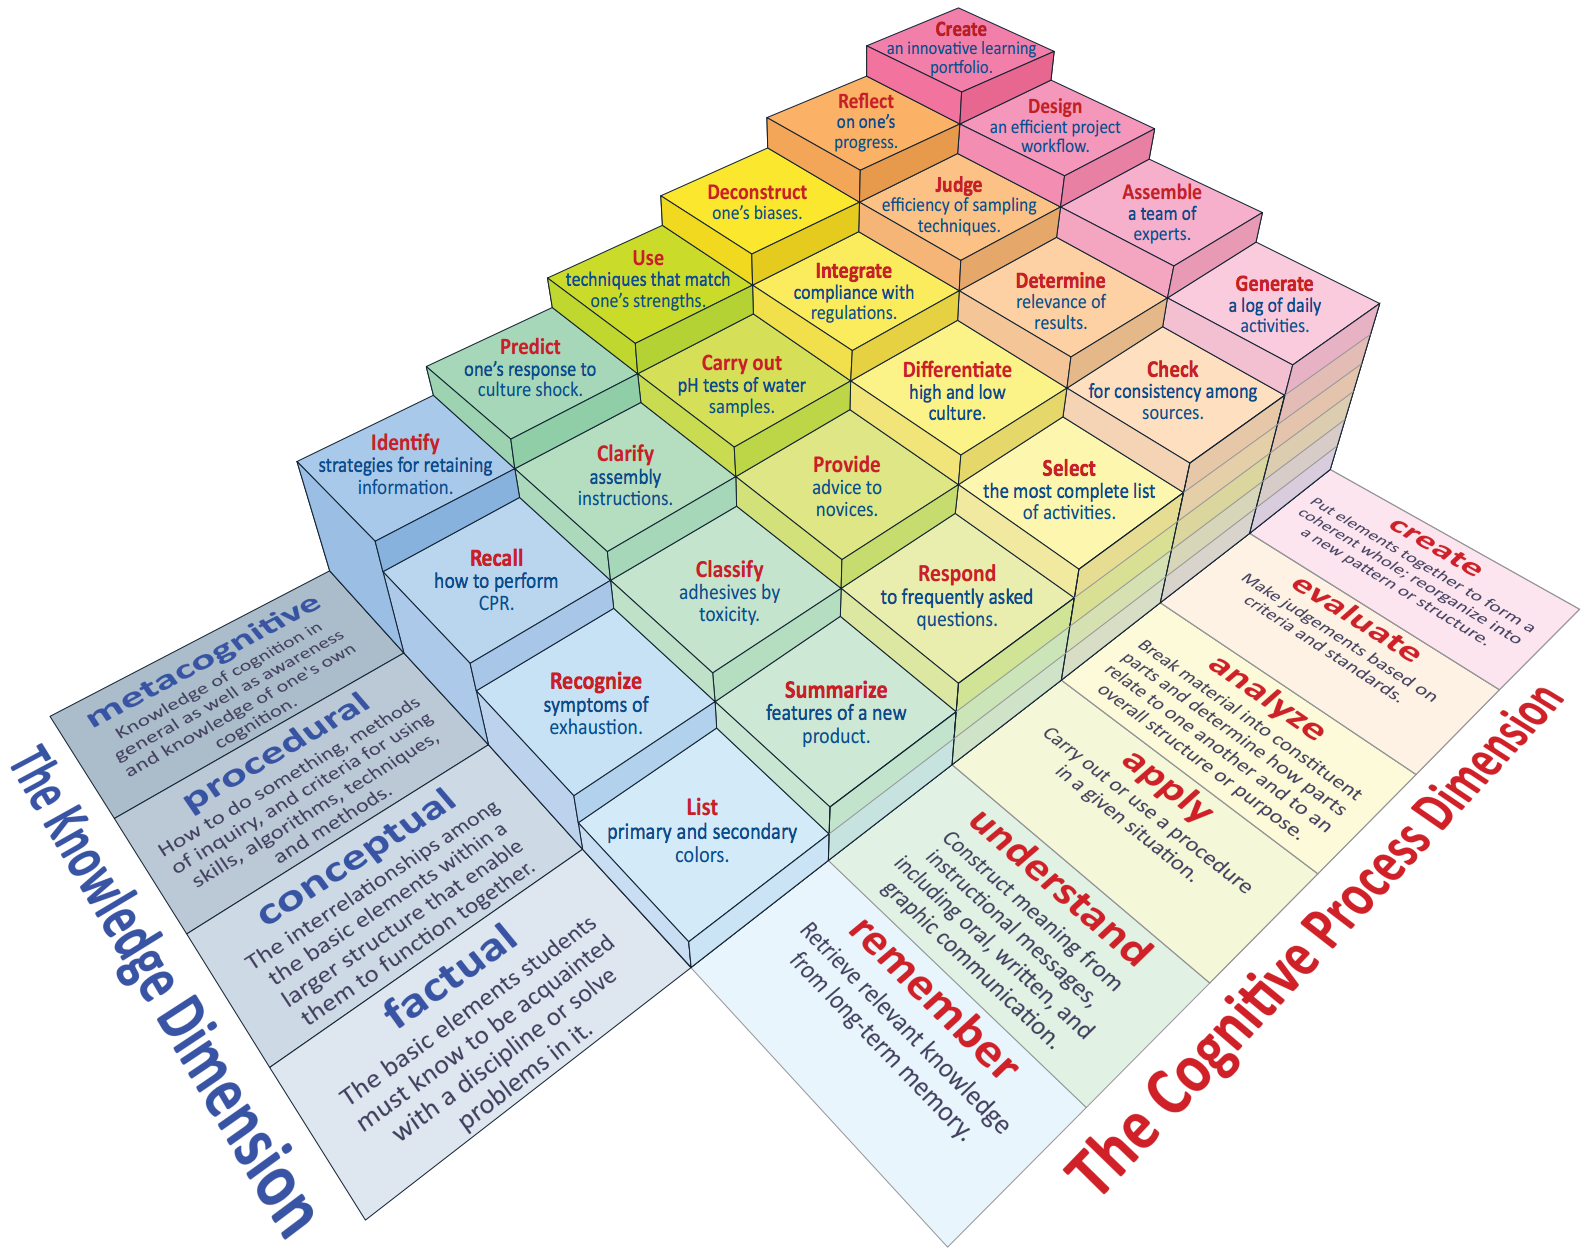
\includegraphics[width=1.0\textwidth]{RevisedBloom.png}
    \caption{Bloom's revised taxonomy visualised with examples of different learning objectives.}
    \label{fig:revised-bloom}
\end{figure}

  Bloom's revised taxonomy can be useful both to map learning objectives for entrepreneurship and as an entrepreneurship coach. To craft good multiple-choice questions could be an art, but to map the question to the learning objective makes it into more of a science:

  Entrepreneurship topic question: "What is financial literacy?" (= \textit{conceptual} and \textit{remember})

  To simulate a procedural environment, the question can be presented as a scenario:

  Entrepreneurship coach question: "It turns out that 10 youth have not carried out the business action, what should you do?" (= metacognitive and evaluating)

  There are several traps that the person formulating the question and answer alternatives can fall into, in the case of multiple-choice, where a good question might be de-amplified because of the answer alternatives.

  Consider the coach being asked to give business advice to a fictional youth named Adam: "Adam wants to start a business that is based on a product. which business should he start?". Before, the coach has been given questions on what a service and product is (factual remember), what the difference is (factual understand), and been given examples (conceptual analyze). Now, the skills are being put to a procedural test.

  If the answer alternatives are obvious (or memorized), the learning will be lower than scoring high on Bloom's revised taxonomy.

  If the answers are high-quality alternatives, all of the answers must be evaluated and considered. In such cases, multiple-choice learning can actually amplify learning, via \textit{learning by repetition} or \textit{learning by thinking}.

  In this case 3-4 valid alternatives might be: "Start a salon", "Start selling soap", "Start a bricklaying business".

  It is still hard to score high on the knowledge and cognitive dimension using techniques such as multiple-choice with entrepreneurship and coaching. This is however necessary, if the app should reach the learning objectives of YoungDrive.

  There may need to be additions to the multiple-choice design, and not only content. Such design ideas may be utilizing flip card techniques (don't see answer alternatives until you've thought of your answer), or asking "How sure are you?", both encouraging metacognitive thinking.

  More ambitious ideas, would be to simulate the entrepreneur coach environment more accurately than via text (using more channels, like audio, video, voice), or to do simulations instead of using multiple-choice. The advantage of multiple-choice, is that data can be collected easily, and that it serves the target group of first-time smartphone users, and because of ease of implementation.

  \subsubsection{Building skills: by Spaced practice, Deliberate practice and Perceptual exposure}

  Spaced practice deals with spreading out learning, with the purpose of not forgetting. E.g. Gates \cite{Gates} concludes that spaced learning versus massed learning (no rest between sessions) did have a memory benefit in their study.

  Taking spaced learning into consideration, could mean making the user apparent on the person's meta-cognitive ability (your personal insight of what you'll remember and when you are likely to forget), and meta-memory (when you need to repeat information in order not to forget).

  Gates \cite{Gates} found no evidence of consistent correlation between total duration and effects on learning outcomes in their study. So how do you design for optimal learning outcomes of skills, particularly if those are entrepreneurial or coaching skills?

  When building skills, Sierra suggests deliberate practice \cite{yengin} \cite{sierra}. The goal is to help users practice right, by designing practice exercises that will take a fine-grained task from unreliable to 95\% reliability, within one to three 45-90-minute sessions.

  Deliberate practice has been proven to be an effective way to build skills. It has also been tested before for mobile learning environments. \cite{yengin}

  Sierra \cite{sierra} suggests skills to be divided into three buckets: can't do (but need to do), can do with effort, and mastered (reliable/automatic). The goal then is to move skills from can't do into mastered, in the best way possible. See figure \ref{fig:sierra-practice} from Sierra \cite{sierra}. Sierra says, if you can’t get the user to 95\% reliability within this time, stop trying; you need to redesign the sub-skill. \cite{sierra}

  \begin{figure}[h]
    \centering
    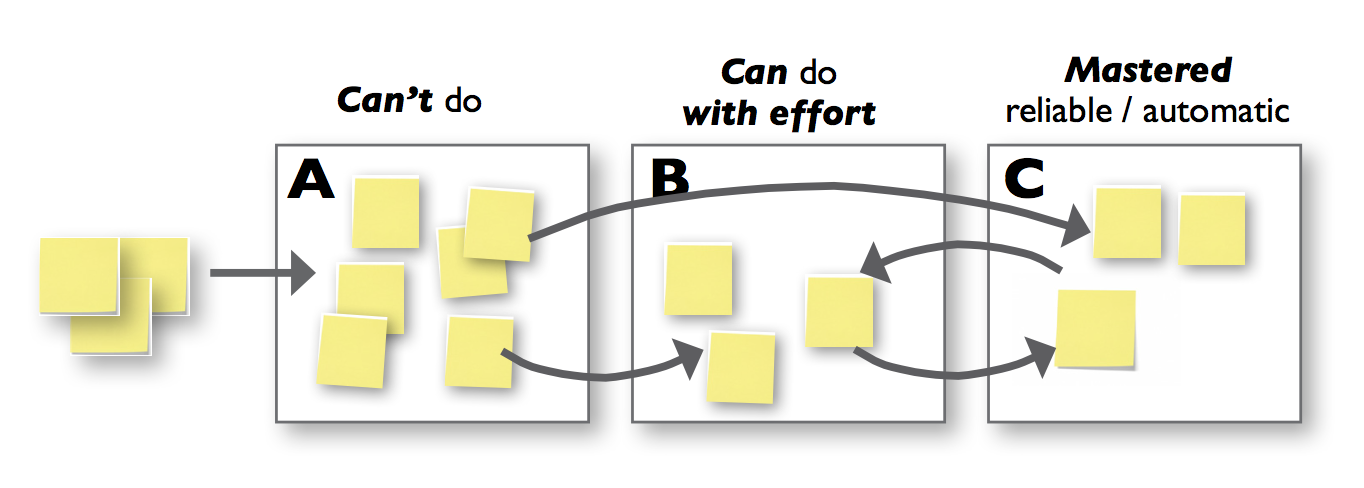
\includegraphics[width=0.8\textwidth]{SierraPractice.png}
    \caption{Moving skills from A (Can't do) to B (Can do with effort) into C (Mastered) can move different ways, depending on how effective the learning is. Deliberate practices focuses on A-B-C, while perceptual expose enables A to C. Reflection allows knowledge to go backwards, to get better at the skill than previously possible. An example might be to teach "Financial literacy". Concepts and factual knowledge (like what income and profit is) might need to move A-B-C, whereas entrepreneurship skills (like taking financial decisions) can move A-C if it becomes intuitive for the user, e.g. via having been exposed to a lot of trial-and-error examples in the app.}
    \label{fig:iterationprocess}
\end{figure}

  Desirable difficulties applies here, meaning that during deliberate practice, it may feel as if learning gets harder and harder, but in the long term the user is actually learning more. As a result, less people does true deliberate practice, but they do not get the same reward in return. This needs to be designed for, e.g. using social psychology.

  By deliberate practice, you can practice better. The second attribute of those who became experts, were that they were exposed to high quality, high quantity examples of expertise. \cite{sierra}

  It shows that whenever a skill relies on intuition, we could try exposing the user a well-designed trail and error test. In the case of multiple-choice questions, this could be done by exposing users to very high-quality samples during a very limited time. Perceptual knowledge includes teaching what we think of as expert intuition (like being a good entrepreneurship coach).

  Sierra shows how researchers have repeatedly, by well designed tests, been able to quickly build expertise by trial-and-error feedback. A novice would hazard a guess and an expert would say yes or no. Eventually the novices became, like their mentors, masters of the expertise that could otherwise would have been intangible for long.

  \subsubsection{Learning from Assessment}

  Knowing what learners know, and don't know, is crucial to effective learning, Luckin \cite{luckin} says.

  Assessment can partly help to design for flow, matching challenge and ability \cite{bruhlmann}, which is effective for intrinsic motivation (see next chapter).

  Moreover, it also has cognitive benefits. It can help to offer appropiate feedback, increase learners' awareness of their learning needs, and give accurate assessment and analysis, and allows learning to be tailored.

  By recognizing differences of students, in their ability to understand what they know and how they can progress, it is possible to ensure that everyone achieves their full potential.

  Effective assessment by a teacher or agent includes individual feedback (task-oriented and informal) and appropiate feed-forward advice.

  \subsubsection{Learning by Thinking: Reflection \& Retrieval Practice}

  Stefano \cite{stefano} suggests that that reflection has been an overlooked area of research for a long time. During the act of reflection, the student develops necessary skills and self-awareness to refine their own learning activities. His results suggests that reflection as an activity that can be more effective than additional learning. This surely applies to the teacher as well, Luckin says. \cite{luckin}

  Stefano found that individuals who are given time to reflect on a task, outperforms students who are given the same amount of time to practice with the same task. But, similar to deliberate practice, it is a desirable difficulty: individuals in the test themselves, had a tendency to believe that allocating time to practice on the task rather than reflecting on it would benefit them.

  %\subsubsection{Retrieval practice}

  When it comes to study technique, Bjork \cite{bjork} as well shows that retrieval from memory is more effective than people who repeat reading the same thing to remember: the more effective students, retrieves from memory.

  One way to use memory retrieval as a study technique, is to ask "What was in that article?", before checking the answer in the article (the flipcard principle). It is an example of memory retrieval that is extremely effective for learning, their research shows. There is a danger with multiple-choice questions, that the student is given no time to reflect on the question and their prior knowledge, before evaluating the alternatives.

%\subsubsection{Not forgetting}

%UCLA Bjork's Learning and Forgetting Lab researches how people forget, and how to design so that people do not forget.

%\include{theory/learning/pedagogical-development/social_psychology}



\subsection{Methods to Design for Motivation}

Social psychology can guide the design, when there is a wish to make people behave differently. A big research area is motivational psychology.

With a compelling context, the users are already motivated. Their motivation, is to become better.

Sierra \cite{sierra}, instead suggests the focus to be how to help users progress (see "Progress and payoffs"), and what pulls them off (see "Cognitive load theory").

\subsubsection{Cognitive load theory}

Sierra argues working on what stops people, matters more than working on what entices them. Thus, a focus needs to be identifying and removing blocks.

Sierra \cite{sierra} describes how humans have scarce cognitive resources, and how to design for these.

Cognitive load theory research is divided into three areas: intrinsic CBT, extrinsic CBT, and germane CBT. Below, to design for these are described.

Intrinsic CBT, needs to be dealt with if the effort is too high. Sierra \cite{sierra}describes two strategies. She first says that according to deliberate practice, if you can not get to 95\% reliability within three 45-90 minute sessions, split skills that can be done with effort into sub-skills. The purpose is to reduce time spent practising being mediocre.

Extrinsic CBT, the way presented to a learner, should be handled via designing to support cognitive resources, Sierra says \cite{sierra}.

Scaffolding is a technique to step by step remove the support wheels for the user, e.g. present information in different ways. Gates' \cite{gates} report shows that in their research, each category of scaffolding demonstrated significant effects on learning.

Also, reduce cognitive leaks by e.g. don't make them memorise, and make the thing you want the user to do, the most likely thing to do (affordances). Everything that takes willpower, reduces cognitive leaks.

Germane CBT, is the work put into creating a permanent store of knowledge. To support cognitive resources, escape the brain's spam filter by making the information essential. Either by designing for the compelling context, or desining for just-in-time learning versus just-in-case, Sierra says. \cite{sierra}

\subsubsection{Progress and payoffs}

Sierra aruges that to pull users forward, to stay motivated, progress and payoffs are essential. Both of these, are investigated in terms of motivational psychology.

The feeling of progress can be emphasised by a path with guidelines to help the user know where they are at each step, e.g. for a training.

The best payoff, is a intrinsically rewarding experiences, according to Sierra \cite{sierra}.

It is superb to gamification, says Sierra \cite{sierra}. This is in-line with self-determination theory, where e.g. Pink \cite{pink} says that the surprising truth about what motivates us is that drive is fostered by autonomy, mastery and purpose. The most efficient way is therefore to design for having intrinsically rewarding experiences.

Caring for the compelling context, why the user wants to learn the skill, are helpful strategies. Other strategies are flow, mentioned before, or to give high pay-off tips, helping the user progress in a fair way.

Gates \cite{sierra} says that simple gamification as well as more sophisticated game mechanics can prove effective. However, they add that it should be investigated if "simple gamification" (e.g. contingent point and badges connected to learning activities) more frequently focus on lower-order learning outcomes, compared to studies with more sophisticated game mechanics.


\subsection{Making users awesome}

Making Users Awesome: "My compelling context: I want to help you become an even better coach. (2016-02-24)

The Better User POV:
Don’t just make a better [X] (coach training app),
make a better User of [X] (coach training material)

Assignent:
Write a detailed description of what you see and hear, for the time-frame that makes sense for your bigger context.
You can do variations of this exercise for users at different levels from first-time newbie to expert.The key is to start thinking—hard—about what most products and services don’t: the post-UX UX. (s. 57)

Create a definition of badass for your context (s. 89)
"Given a teaching situation among the youth group, a great coach can teach an entrepreneurship topic more consistent with what the coach material said."

Create a definition of badass for your context (s. 90)
"Given a question in the app, a badass user of the coach training material will get the right answer more often, and leverage the correct answer to their coach situation."

\textbf{Simplified rules for Deliberate Practise}
Help them practice right. Goal: design practice exercises that will take a fine-grained task from unreliable to 95\% reliability, within one to three 45-90-minute sessions

If you can’t get to 95\% reliability, stop trying! You need to redesign the sub-skill

\textbf{Perceptual exposure}
With a little ingenuity, the British finally figured out how to successfully train new spotters: by trial-and-error feedback. A novice would hazard a guess and an expert would say yes or no. Eventually the novices became, like their mentors, vessels of the mysterious, ineffable expertise.

Perceptual knowledge includes what we think of as expert intuition. (like being a good coach) Thus, we should expose him/her to trail and error via the coach training app.

\textbf{Create a path (s. 193)}
Make a list of key skills ordered from beginner to expert, then slice them into groups to make ranks/levels. For motivation, the earlier, lower levels should be achievable in far less time and effort than the later, advanced levels. One possibility is to have each new level take roughly double the time and effort of the previous level.

\textbf{Exercise: design a “belt” path for your context (s. 197)}

\textbf{Exercise: What’s the first “superpower” for your context? (s. 205)}
Like going up a rank?
A hint of becoming a Certified coach

\textbf{Just-in-Time learning (vs. Just-in-Case)}
To bypass the brain's spam filter.

\textbf{Validate the need for this knowledge - What knowledge goes on the board?}
topics on trial, and mapping to skills.

s. 271 jätteviktig

1. Compile the cards of initial knowledge and skills

2. Map the knowledge to a skill and verify that you \textit{can’t} possibly do this skill without this knowledge

3. Remove orphaned (unmapped) knowledge. Never forget cognitive resources are scarce and limited.


\subsection{Design Thinking}

%\subsection{Digital Learning}

%\citep{edtech-clark}
%\citep{edtech-sjoden}
%\citep{edtech-dangelo}

\subsubsection{Mobile Learning}

\textbf{The use of deliberates practices on a mobile learning environment}

TODO, superbra artikel

\textbf{An experiment for improving students performance in secondary and tertiary education by means of m-learning auto-assessment}

Luis de-Marcos

% Proved successfull, everyone improved their knowledge. I can use a similar methology, and compare to the development context.

--

Huang et al. (Huang et al., 2008) indicated the common problems encountered in m-learning applications: (1) software integration, (2)
limitations of the web browser, (3) interface usability, (4) reduced size of the screen, and (5) limitation of the battery life. Such limitations are
of particular relevance when the application is intended to run on students’ personal phones; in this case, decisions need to be taken in an
attempt to alleviate the impact such issues may have. Of the problems listed above, item 2 can be mitigated by developing a mobile
application that does not run on the web browser. Items 3 and 4 can be alleviated by designing an interface that minimizes the amount of
information displayed and the input required from the user. This was the main reason for preferring multiple-choice questions to other
kinds of questions, since these questions can usually be stated in a few lines and require the selection of one or more choices. A few mobile
phone buttons can then be programmed to select/unselect each option. Moreover, various experimental studies (Chen, 2010; Ventouras,
Triantis, Tsiakas, \& Stergiopoulos, 2010) support the validity of this assessment method. Solving the problem represented by item 5 was
beyond the scope of this study; however, students were advised to charge their devices before taking the tests and teachers were advised to
design tests of no more than approximately 10 questions, in order to reduce connection times to a maximum of 20 min. Finally, item 1 was
especially difficult to tackle. When the technological framework was set up, our decision was to define the minimal software requirements
that handheld devices would have to meet in order to run the application.

% NTA Digital, Om Digitalt Lärande, Att lära med digitala verktyg
% http://ntadigital.se/teacher/tutorings/2

Interaction design talks about the creation of digital artefacts specifically. When it comes to the design process, it is influenced by related areas such as human-computer science, and more recently human-centred design. However, various disciplines suggests different design processes. For example, agile development suggest how do develop software efficiently. Whenever a project is multi-disciplinary, various design processes may need to be combined. Whenever this happens, design thinking (how to think about design) becomes a skill essential to thoughtfully design the process.

\cite{lowgren} writes about design thinking and useful techniques in general, from his interaction design perspective. Service design thinking connects various fields of activity \citep{stickdorn}, and it's methodology relies on being close to the users. While interaction design talks about the creation of digital artefacts specifically, service design talks about the creation of services. As some digital artefacts are used within a service, or can be thought of as both a product and service simultaneously, the combination of the two can be very useful. Service design could help the designer be aware of how such a artefact would need to interplay with its physical environment.

Each discipline holds efficient methods and tools, that can be modified to suit the specific situation even better. From the field of graphic design, mental models describes the perceptions of the user. From interaction design, desirability, utility, usability and pleasurability can be useful principles to evaluate a product. While none of these are a mandatory part of service design, these have been useful in service design projects previously \citep{stickdorn}. In difficult situations, combining different disciplines places demands on the designer. This is where design thinking becomes relevant. Below, relevant methods and tools are briefly described, and what it means to be a good designer.

\subsubsection{A Good Designer}\label{aGoodDesigner}

The result of a method can not be better than the people engaging in carrying out the process \citep{lowgren}. With its user-centered focus \citep{stickdorn}, service design can be said to equip the designer with tools both for reasoning and design ethnography. But it also suits to get to know and design for the learning situation. In learning, the end goal is that the student raises their level of knowledge and expertise, and the design needs to be adapted for this specifically. Central to design for learning is to dig deep into the topic being communicated. In this case, understanding entrepreneurship, understanding exactly what is being taught (the training), and adapting the design after this.

A good designer can deal with the complexities of design: a satisfactory (and surprising) solution or design can be achieved while working in a highly restricted situation \citep{lowgren}. This can be done e.g. by inventing new design techniques. One such example that would suit designing an app for entrepreneurship training in a development country, would be a \textit{field hackathon}. A field hackathon would thus allow that during the training, the topic \textit{and} the users are observed and understood. Then, the app can be tested (in this can a quiz assessment of the trained material). Then, users can be invited to give feedback, suggestions of improvements, and  ideas. For the next day, an improved version of the app is tested, and then the process is repeated.

More examples of how a service design process can be invented to deal with digital artefacts, can be desribed in the chapter \ref{digital-service-design}. However, to do such field tests (like a field hackathon), requires building trust and having an enabling environment, which is where relationships and roles becomes crucial.

\subsubsection{How to Deal with Relationships and Roles}
While a researcher is interested in reality, a designer is interested in what reality could become \citep{lowgren}. Being thoughtful means conceptual clarity from the designer, caring for the vision, and being equipped with appropriate tools of reasoning. These are all good characteristics for a successful project. According to \cite{lowgren}, "real" design is about finding ways to design a project within the existing preconditions and limitations. Being innovative and communicating well with the stakeholders becomes crucial.

There are three roles as interaction designer in particular can take: the computer expert, the socio-technical expert, and the political agent. The trend is increasingly towards socio-technical experts \citep{lowgren}, the middle ground, as human understanding and collaboration is so important. This seems to be a perfect fit with service design, where interaction design is both technical skills and design, and service design can be both design and ethnography. Even more importantly, service design suggests making the whole process co-creative, involving all stakeholders \citep{stickdorn}.

\subsubsection{Thinking of a Product as a Service}

Service design thinking is described as a process of designing, rather than to its outcome. A service's intent is to meet customer needs. If it does, it will be used frequently, and recommended \citep{stickdorn}. As this is often not the case, service design can be applicable to fields including social design, product design, graphic design and interaction design. The result can be a product service hybrid. When designed and considered well, service design shapes the value proposition and desirability of the product for the better.

\subsubsection{Starting the Project}

\cite{lowgren} writes about the beginning of a project: This is where the designer gets involved in design work, establishes a preliminary understanding of the situation, navigates through available information, and initiates all neccessary relationships with clients, users, decision makers, and so forth. Based on all this, she creates a design proposal \citep{lowgren}.


\subsection{Service Design Methodology}

Below, brief descriptions of five principles of service design are described according to \cite{stickdorn}, together with how the work is divided into iterations, and examples of tools that can be applied.

\subsubsection{Principles}
\cite{stickdorn} describes five principles that constitute service design thinking, and how to follow these.

He describes how to follow these principles, by making the process user-centered (e.g. via \textit{design ethnography}), co-creative (involve all stakeholders) and holistic (keep the big picture). Sequencing (visualize the service, and make iterations) and evidencing (make the service tangible) are the two last important principles.

\subsubsection{Sequencing}
Sequencing the process means splitting the design process into iterations, which consists of a number of steps, which are repeated for each iteration. This is a common denominator with the agile methodology SCRUM, which is often applied in software development.

While service design literature and practice refer to various frameworks, regardless of number of steps, every service design project includes: exploration, creation, reflection and implementation \citep{stickdorn}. \citep{expedition-mondial} suggests a model where one iteration consists of insights, ideation, trigger material, and interactions. See figure \ref{fig:iteration}.

\begin{figure}[h]
    \centering
    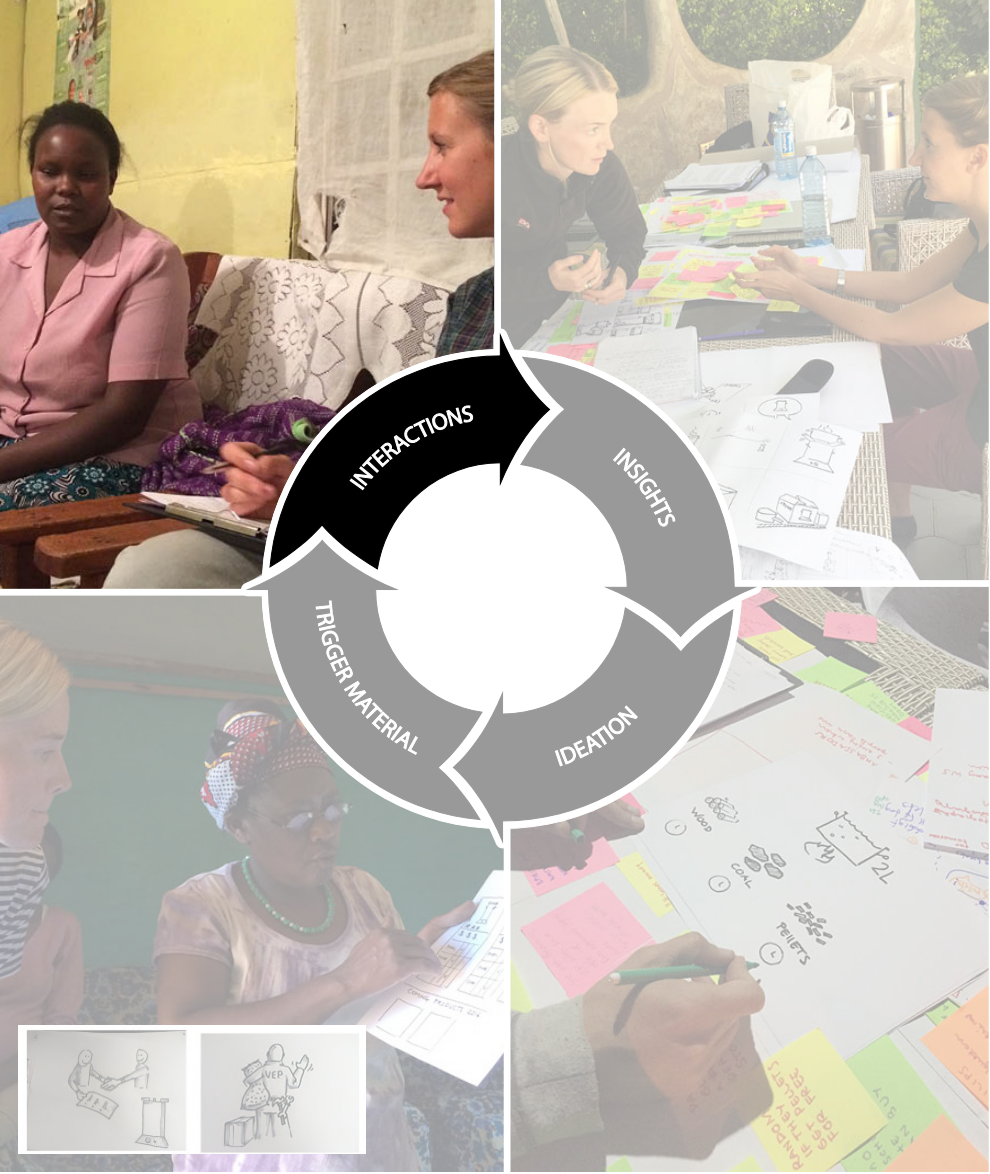
\includegraphics[width=0.7\textwidth]{Iteration.png}
    \caption{In Nissar's model, a iteration consists of Interactions, Insights, Ideation and Trigger material.}
    \label{fig:iteration}
\end{figure}

\begin{enumerate}
\item Interactions, where you are listening, the \textit{Explorative phase}.
\item Insights, which is where you use the Interactions in order to try to understand, the \textit{Understanding phase}. % better word+
\item Ideation, where you find possible ideas and when creation of new version of the app is done, the \textit{Design phase}.
\item Trigger material, where material is developed to test the outcome of our evaluation in the next round, the \textit{Trigger development}.
\end{enumerate}

The iterations should come closer and closer to a desired outcome. It is not always obvious what this outcome is. For each iteration, the process takes the project closer, from Why? to What? to How?, often with overlaps \citep{expedition-mondial}. See figure \ref{fig:iterationprocess}.

%\begin{wrapfigure}{r}{0.25\textwidth} %this figure will be at the right
%    \centering
%    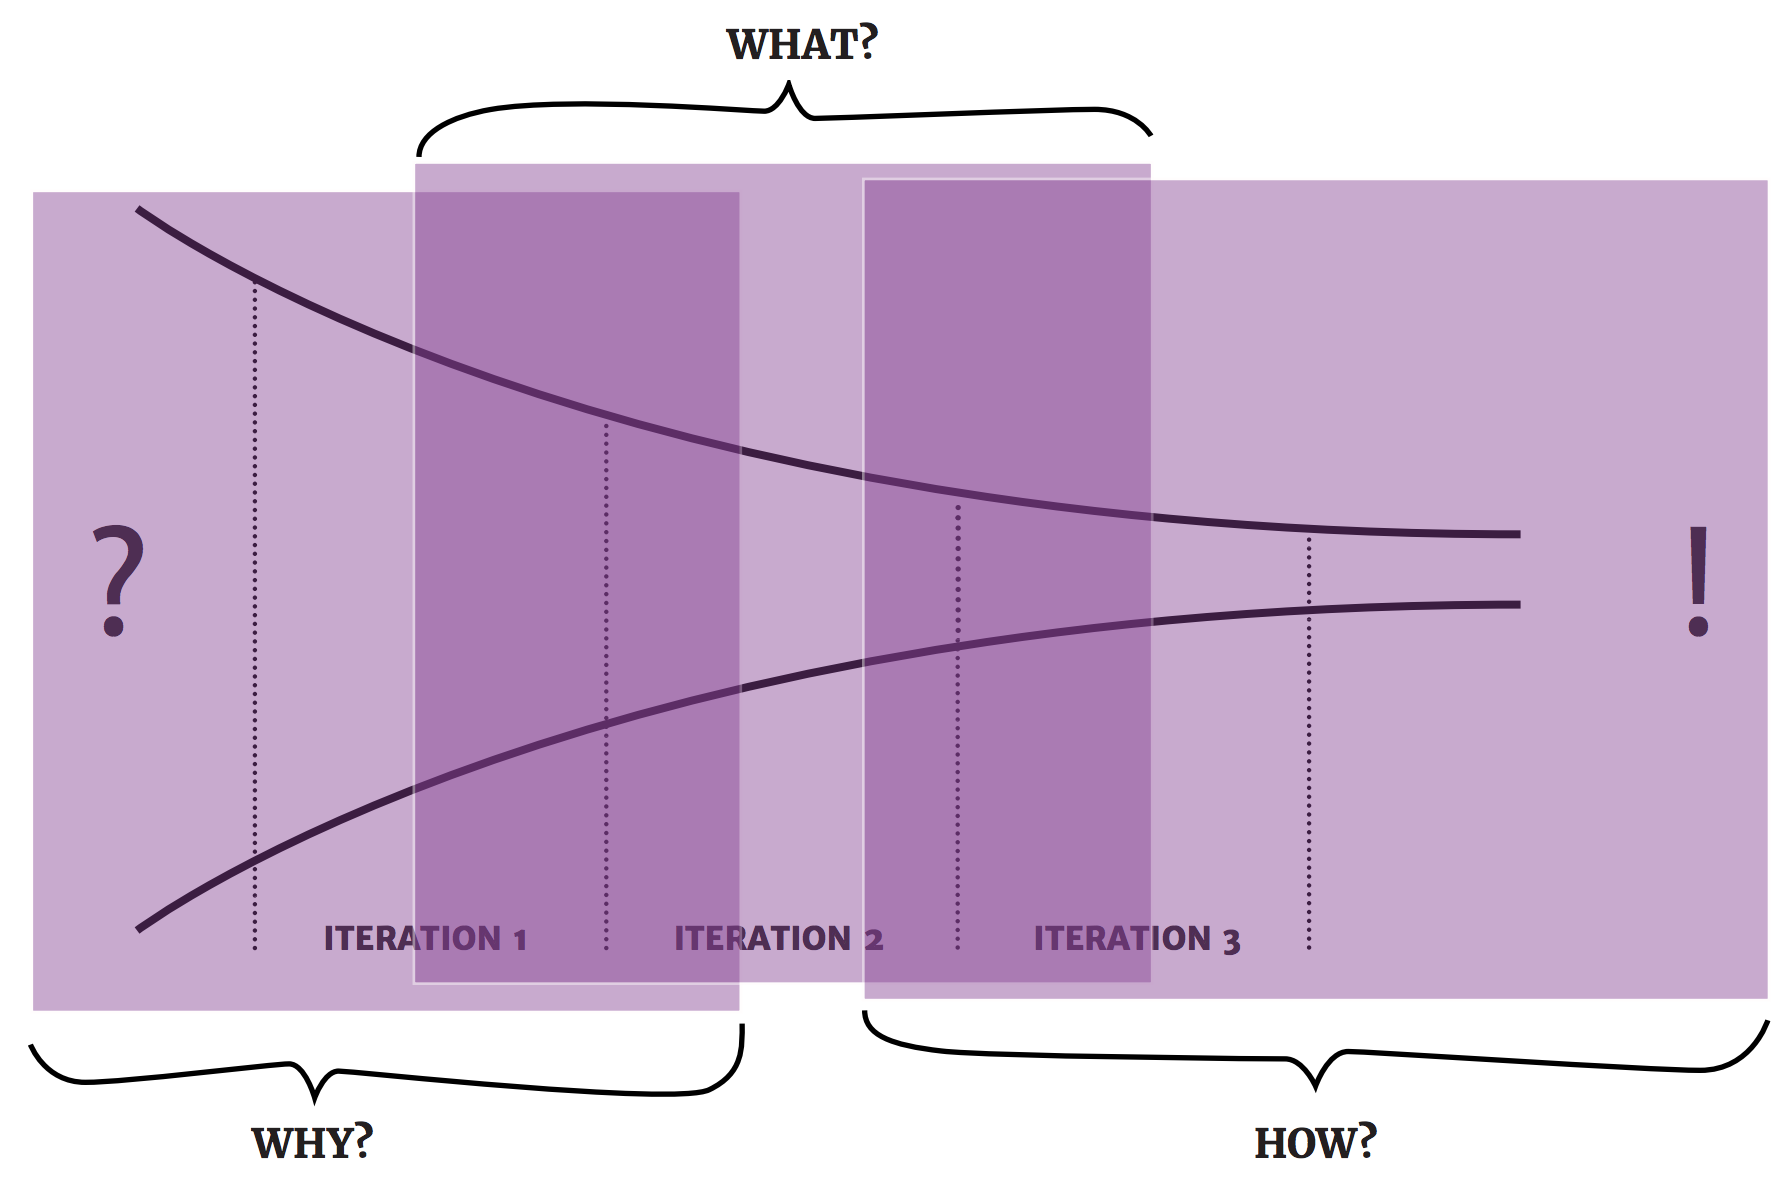
\includegraphics[width=0.25\textwidth]{IterationProcess.png}
%    \caption{Iteration process}
%    \label{fig:iterationprocess}
%\end{wrapfigure}

\begin{figure}[h]
    \centering
    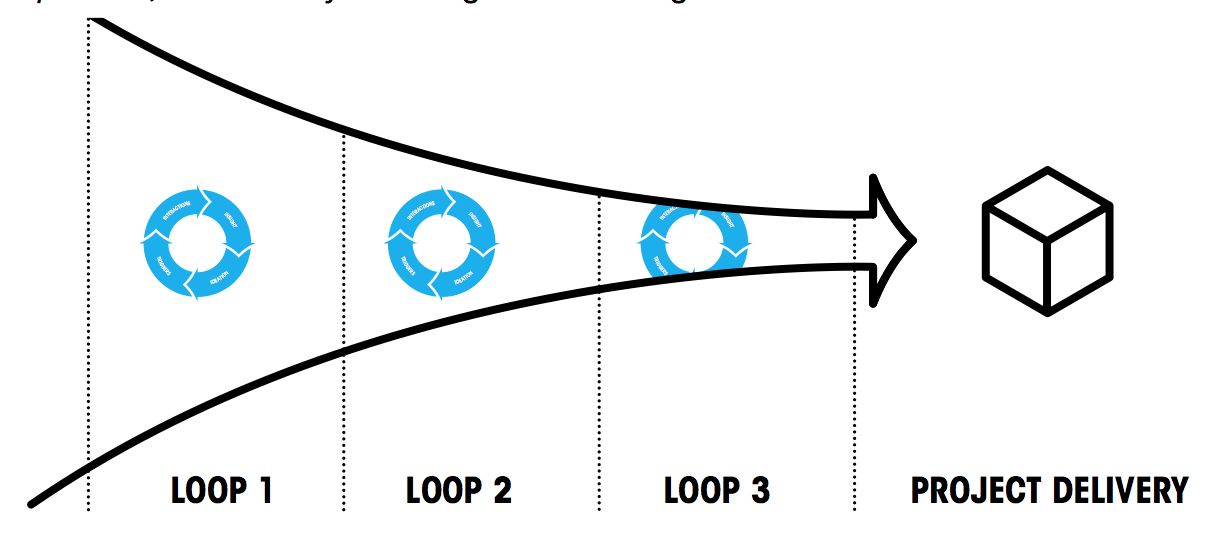
\includegraphics[width=0.8\textwidth]{projectLoop.png}
    %IterationProcess.png
    \caption{The iteration process consists of a number of iterations with different focus, starting with broad strokes, and narrowing down into a concrete product. Between iterations, there is an overlap in "Why?" and "How?", "How?" and "What?", which signals that there is a learning process which means conclusions may need to be quickly questioned as new insights emerge. This is especially important in projects where you work with an unfamiliar target group and there are several uncertainties and constraints.}
    \label{fig:iterationprocess}
\end{figure}

\subsubsection{Service Design Tools}

There are a number of popular service design tools that follows the five principles, e.g. how to make it user-centered. One is Customer Journey Map, in which an activity (like hosting a youth session) is broken into Before, During and After. Another method is Personas, which \textit{exemplifies} thought users of the app into people with names, having realistic character traits and opinions. The persona's neeeds can then be thought of when designing. An alternative to Personas are Need groups, where thought users are broken down by their different needs. Instead of designing for a specific person, you design for a person with a specific need. The advantage of Need groups, are that it accepts the view that the same person (Persona) might have different needs, depending on situation. The 5 Why's is a simple method used to dig deep into understanding the interviewee. Variants of the question "Why?"" is repeated five times as a rule of thumb, to understand underlying motives. This method is called "Why-why-why" within interaction design \citep{lowgren}).

Tools to create and reflect can be done via certain work methodology. When you structure and inspire brainstorms, you can ask "What if...?" and do Co-Creation, meaning doing ideation together with stakeholders or users. To create, agile development can be used, which is often suitable for software engineering. The manifesto for agile development is \citep{agile-manifesto}:

\begin{itemize}
\item Individuals and interactions over processes and tools
\item Working software over comprehensive documentation
\item Customer collaboration over contract negotiation
\item Responding to change over following a plan
\end{itemize}

An example of an agile methodology is \textit{SCRUM}, where a project is divided into several iterations similar to a service design approach of sequencing, but also introducing consepts like retrospectives (reflecting on one's work) and sprint demo (demonstrating the results of the iteration to stakeholders) \citep{kniberg}.

There are also some service design best practices: interviews are often done via open questions (encouraging stories) and dialogue can be facilitated with a questionnaire guide. In workshops, post-its are often used, and followed up with specific questions. Service design methodology encourages taking pictures, filming and recording audio, benefiting the analysis done afterwards \citep{expedition-mondial}.

%\subsubsection{Relevancy within Social Innovation}
%\citep{socialinnovation-ehn}

%\subsubsection{Service Design Thinking}

%\subsubsection{Methodology}

\textbf{The iteration process}

The time in Uganda is divided into three iterations. For each iteration, the result becomes more and more clear. In iteration 1, there is a very broad scope, without digital focus whatsoever, where iteration 2 and 3 gradually introduces the digital solution. See figure \ref{fig:iterationprocess}.

%\begin{wrapfigure}{r}{0.25\textwidth} %this figure will be at the right
%    \centering
%    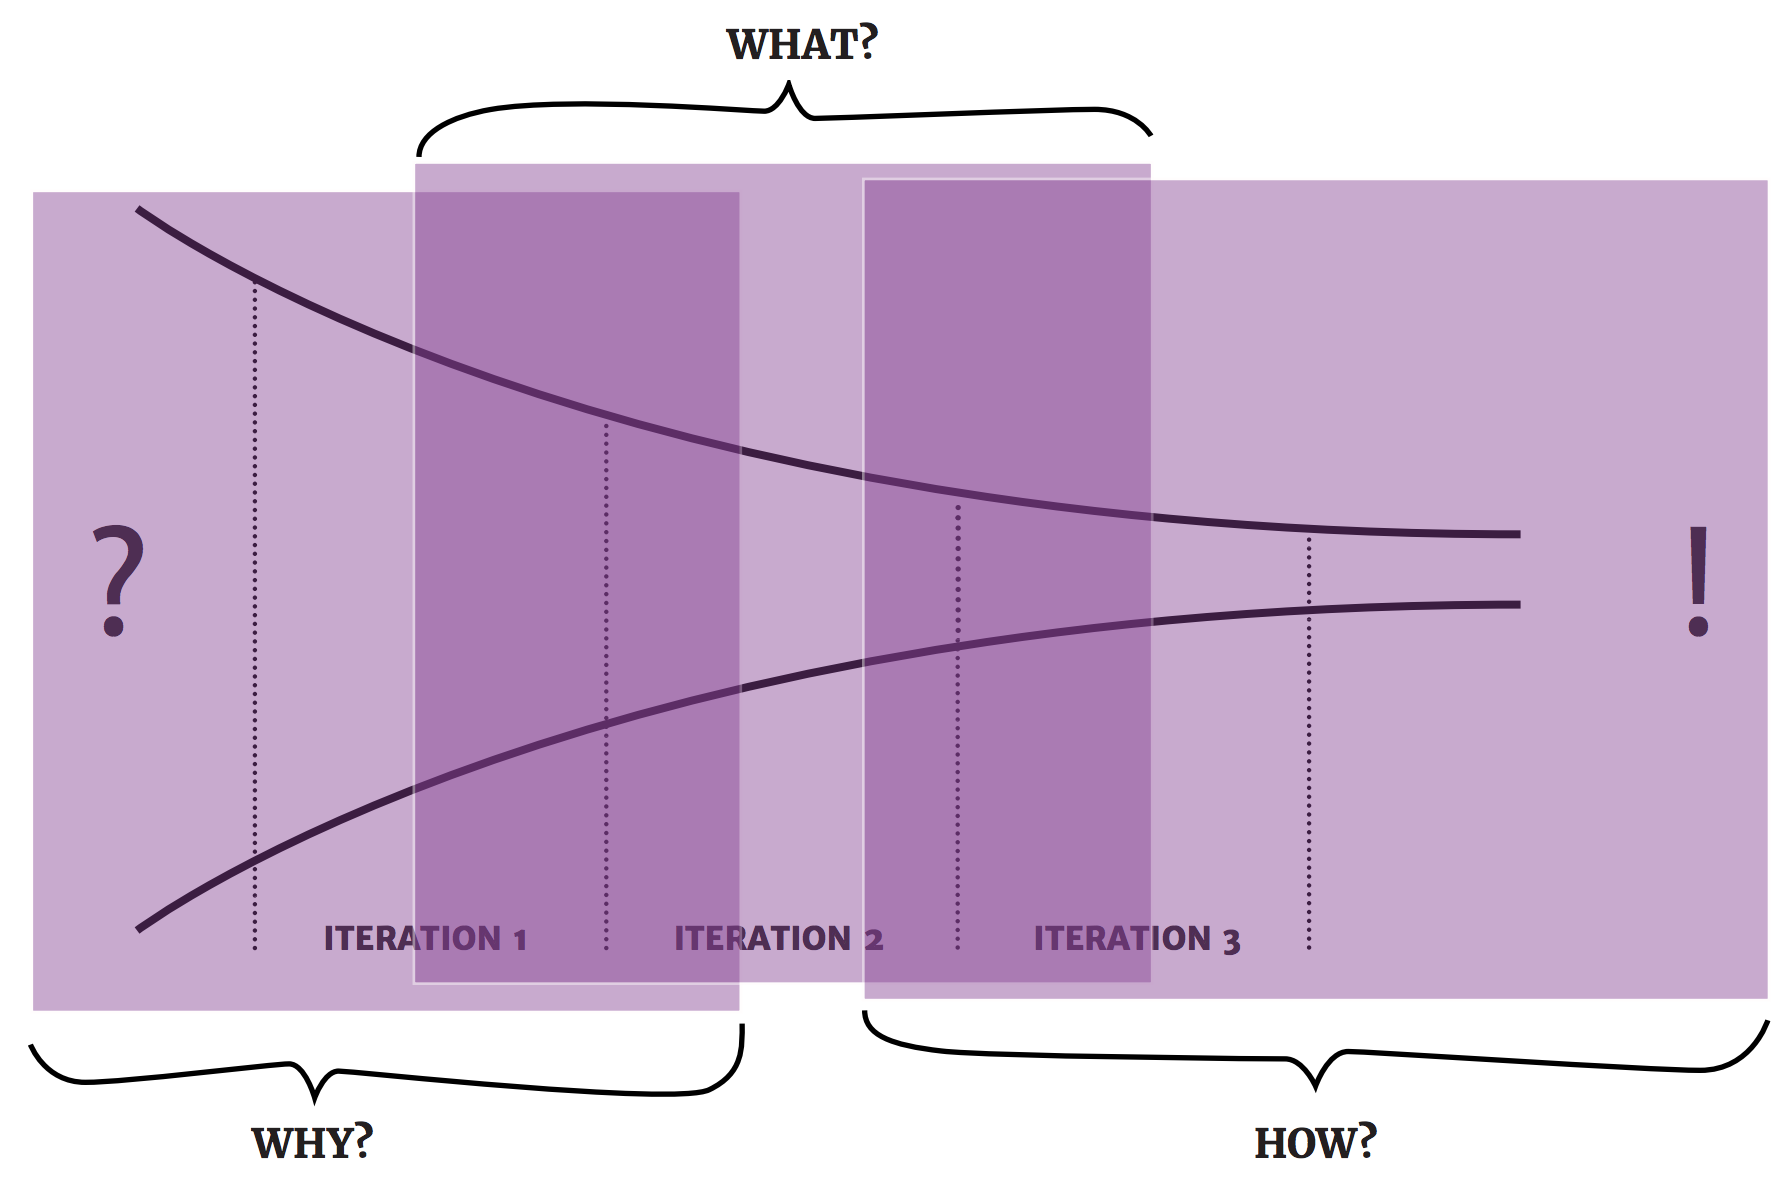
\includegraphics[width=0.25\textwidth]{IterationProcess.png}
%    \caption{Iteration process}
%    \label{fig:iterationprocess}
%\end{wrapfigure}

\begin{figure}[h]
    \centering
    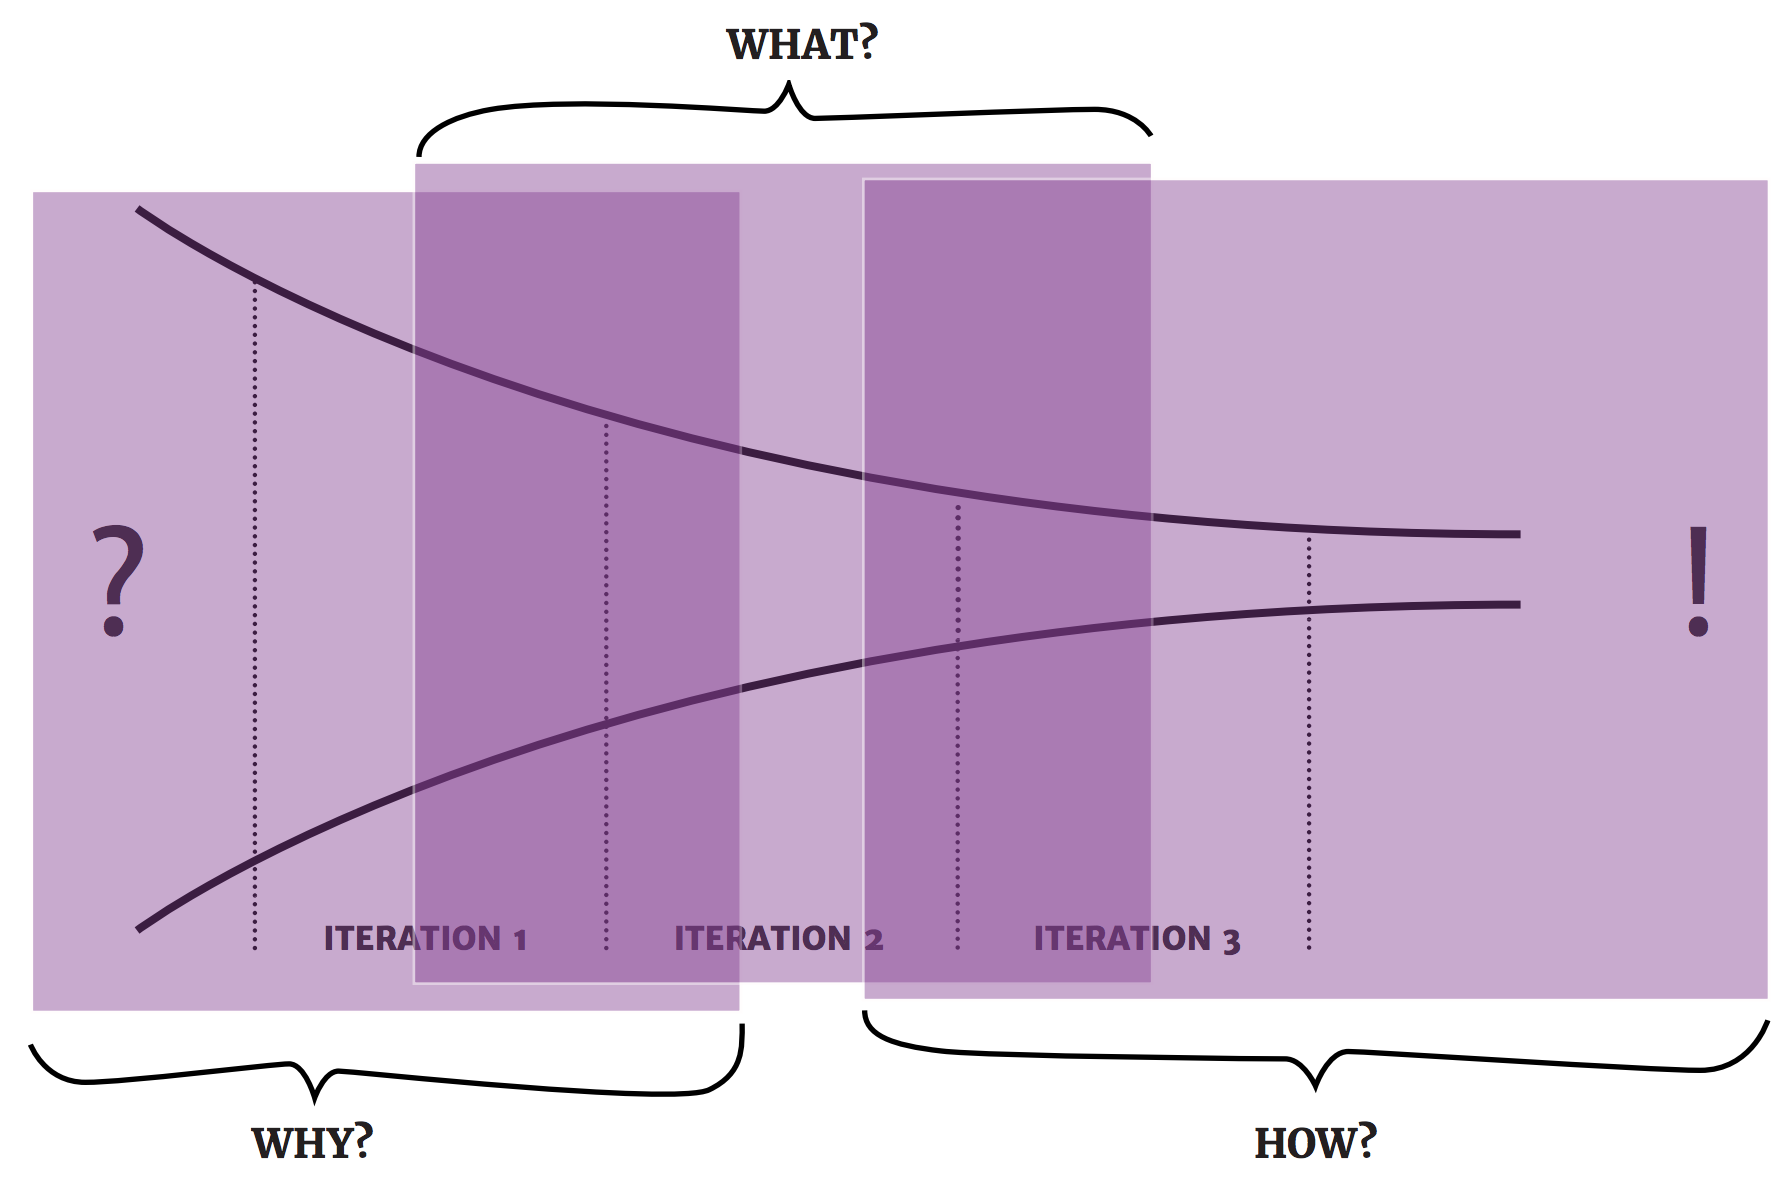
\includegraphics[width=0.8\textwidth]{IterationProcess.png}
    \caption{The iteration process consists of a number of iterations with different focus, starting with broad strokes, and narrowing down into a concrete product. Between iterations, the overlap between "Why?" and "How?", "How?" and "What?", signals that there is a learning process which means conclusions may need to be quickly questioned as new insights emerge. This is especially important in projects where you work with an unfamiliar target group and there are several uncertainties and constraints.}
    \label{fig:iterationprocess}
\end{figure}

\textbf{One iteration} \\
In the way of reasoning around development and design for learning, the steps for each iteration, see figure \ref{fig:iteration}, might be translated into:

\begin{enumerate}
\item Interactions, where you are listening, the \textit{Explorative phase}. 
\item Insights, which is where you use the Interactions in order to try to understand, the \textit{Understanding phase}. % better word+
\item Ideation, where you find possible ideas and when creation of new version of the app is done, the \textit{Design phase}.
\item Trigger material, where material is developed to test the outcome of our evaluation in the next round, the \textit{Trigger development}.
\end{enumerate}

%\subsection{Service Design}
%\citep{servicedesign-ruth},
%\citep{servicedesign-balis},
%\citep{servicedesign-ruth}
%\citep{servicedesign-ideo}
%\citep{servicedesign-stickdorn}

\textbf{The purpose}
Applying service design serves two purposes:

Going from being a computer expert into a socio-technical expert,
In particular, the approach of service design refers to the process of designing rather than to its outcome. (This is Service Design Thinking, 2010, s. 7). ("The outcome of a service design process can have various forms: rather abstract organisational structures, operation processes, service experiences and even concrete physical objects.")

\textbf{The need for service design (in my project)}

\textbf{About service design}
Since service design is a still young and emerging approach, service design education is even younger and just developing. (TISD, 2010)

Without a doubt, you cannot learn what service design is and how to do it just from a textbook. You need to try, fail, learn from your mistakes, improve, try again and thus educate yourself.

Service design education is therefore rather a kind of briefing and tutoring process. Besides explaining the big picture, it is all about giving hints, proposing methods and tools, and showing how to use them while working on a project.

Service design as a practice generally results in the design of systems and processes aimed at providing a holistic service to the user.

Service Design helps to innovate (create new) or improve (existing) services to make them more useful, usable, desirable for clients and efficient as well as effective for organisations.

Service design is all about making the service you deliver useful, usable, efficient, effective and desirable. (UK Design Council, 2010)

(kan lägga till bild)

What distinguishes service design is:

5 principles of service design thinking
Marc Stickdorn
1. User-centred
Services should be experienced through the customer’s eyes. 2. Co-creative
All stakeholders should be included in the service design process.
3. Sequencing
The service should be visualised as a sequence of interrelated actions.
4. Evidencing
Intangible services should be visualised in terms of physical artefacts.
5. Holistic
The entire environment of a service should be considered.

According to TISDT (2010), there is the Customer, Service Provider, Stakeholder, and the Service Designer.

There is then the Touchpoint (every contact point between a customer and the service provider), Service Evidence (a tangible artefact related to a service process), and Service Period (pre-service / service /post-service --current period of a service).

% Här är jag nu i exjobbsrapporten - HÄR

\textbf{How to make it user-centered: TISDT (2010) and Contextual Design (X)}

Agree on a common language!

services are created through interaction between a service provider and a customer. The inherent intention of a service is to meet the customer’s needs and, as a result, be used frequently and recommended heartily. This is often not the case.

Though statistical customer descriptions are important, a true understanding of habits, culture, social context and motivation of users is crucial. We need to put the customer at the centre of the service design process. This requires a genuine understanding of the customer beyond mere statistical descriptions and empirical analyses of their needs. Gaining authentic customer insights includes the application of methods and tools that enable the service designer to slip into the customer’s shoes and understand their individual service experience and its wider context. We are all customers – though with different needs and mindsets. The understanding and disclosure of these disparate mindsets is where service design thinking begins.

we all have individual backgrounds and experiences. The ability to make use of this knowledge during the development of services is crucial for its later success. A user-centred approach offers a common language we can all speak; the service user’s language.

\textbf{Making it co-creative}

This is co-creative.
A broad understanding in various disciplines and a deep knowledge in a specific field is crucial for co-creative work in interdisciplinary teams.


Putting the customer at the centre of a service design process involves facing the reality that potentially there is more than just one customer group, and each group possesses different needs and expectations.
Furthermore, providing services also demands consideration of the various stakeholders,

How can we integrate the stakeholders of a service into the process of designing it?

There are a variety of methods and tools for gaining genuine insights from different user perspectives in the creation of services and for the development, prototyping and testing of these service concepts. This is co-creation, and facilitating this in groups representative of your stakeholders is a vital aspect of design thinking and a fundamental part of service design.

co-creation during the design process facilitates a smooth interaction between the stakeholders during the actual service provision – essential for both sustainable customer and employee satisfaction. Through co-creation customers get the chance to add value to a service in partnership with the service provider early in the development of the service. The more a customer gets involved in the service provision, the more likely this service is of evoking co-ownership which in turn will result in increased customer loyalty and long-term engagement.

\textbf{Making it into sequences} %Chapter: It is sequencing

This is Sequencing.
The series of interactions outline a so called customer journey through the offerings of the respective service.

Imagine a very simple example of a service such as going to a hairdresser. Now try to visualize this service process as
stage play or movie. This movie would consist of a series of static pictures, which would be combined to create a moving sequence. Service design thinking uses this analogy to deconstruct service processes into single touchpoints and interactions. These, when combined, create service moments. Touchpoint interactions take place human-human, human-machine and even machine-machine, but also occur indirectly via third parties, such as reviews from other customers or via print or online media.

Every service process follows a three-step transition of pre-service period (getting in touch with a service), the actual service period (when the customers actually experience a service) and the subsequent post-service period.

Like a stage play, a service moment not only consists of what is happening front of stage, it also includes multiple backstage processes such as cleaning of the shop
33
floor to prepare the front of stage for action. To achieve an excellent theatrical performance, actors have of course to run through many rehearsals; services are no different. We need to prototype services and iteratively test their impact on customers.

\textbf{It is evidencing}

% OBS: korta ner! Ta inte mer så mycket av detta i teorin, för det blir jobbigt att följa upp på.

Make the intangible tangible!

Services often take place unnoticed in the background, like the housekeeping service in a hotel. In fact, services like these are intentionally designed to be inconspicuous. However, if paying a bill is the first moment customers become aware of such backstage service processes, their inconspicuousness might create a disparity in customer expectation and potentially result in their disaffection with the service.

Physical evidence or artefacts such as souvenirs or small bottles of shampoo from your hairdresser can trigger the memory of positive service moments and thus, through emotional association, continue to enhance customers’ perceptions of the service they have received.

Service evidence can thus prolong service experiences beyond the mere service period far into the post-service period. Utilising this effectively has the potential to increase customer loyalty and for customers to recommend the service to others. %Här finns en uppenbart grym koppling till Badass: Making Users Awesome!

In addition, evidence can explain certain aspects of a service touchpoint or process, a sign next to an electric hand dryer pointing out that the proprietor knows that customers would prefer to use real towels but that costs or the environmental impact do not allow this can generate appreciation and empathic engagement.

Evidencing can occur in a variety of forms: bills, mail, emails, brochures, signs, souvenirs or other pro-ducts. These add a tangible component to what would otherwise have been an intangible experience.

Service evidence needs to be designed according to the service’s inherent story and its touchpoint sequence. If a service process is like a movie, a better understanding of the work behind the scenes (i.e. the backstage processes of services) can result in an increased customer appreciation of the service experience.

\textbf{It is holistic}

Keep the big picture!

Which aspects need to be considered when designing services?

the intention should always be to see the wider context in which a service process takes place.

At the level of individual touchpoints and service moments, the focus should be on the environment where the service takes place. The conscious awareness of what customers might otherwise perceive subconsciously with their senses can have a profound impact on the experience of the service itself.

% Detta kanske jag inte tar med?
At the level of the service sequence, there should be a focus on alternative customer journeys. There are always a number of alternative touchpoints and approaches, which need to be taken into account. Sequences change and need to be repeatedly reappraised from various perspectives to ensure a great customer experience. Hence, it is important to map the mood and feelings of all stakeholders throughout the service journey.

To summarise, service design thinking supports the co-operation of different disciplines towards the goal of corporate success through enhanced customer experiences, employee satisfaction, and integration of sophisticated technological processes in pursuing corporate objectives.

\subsubsection{Who are these Service Designers?}

Service design thinking as an interdisciplinary approach includes and connects various fields of activity.

\textbf{Product Design: developing products with service applications (TISD, s. 50)}
This chapter looks at the influences of service production upon product design and considers the implications of the evolution of product designers from designing just products to designing services too.

Design is arguably now focused on the interaction between people and technology, and products serve as platforms for experiences, functionality and service offerings (Buchanan, 2001).

Designers study users and their usage of artefacts to develop better products and generate knowledge that can be embedded into artefacts.

Users generate knowledge through interpretation of this embedded knowledge in artefacts. They need to be able to understand the value, meaning, and the ways to use the artefact in different situations of their daily lives.

\subsubsection{This is co-creative}

The concept of activity refers to participants’ interactivity, initiative and style of collaboration and contribution in design events. User roles may vary from proactive participation where users contribute to solving and framing design challenges to passive roles where designers instead interpret user data without any direct engagement with the user community (Keinonen, 2009).

\textbf{Iterative design development} helps to solve problems found in user testing. There must be a cycle of design, testing and measurement, then redesign, repeated as often as necessary. This is a way to incorporate results of behavioural testing into the next version of the system. Making a system user friendly and easy to operate is the goal of this approach (Gould and Lewis, 1985). Iterative design is a design methodology based on a cyclical process of prototyping, testing, analysing, and refining a work in progress.

Both conceptual and iterative design approaches are important phases in the service design process. The challenge is to design user-orientated hybrids that incorporate both the customer facing products and that help articulate the service they assist in offering.

\textbf{Product-service hybrids}

Koivisto (2007) defines hybrid products as products where the service has been designed as an inseparable part of the product. % A good example of this is Apple’s iPod and iTunes product package (Apple, 2010). Developing such a hybrid product means that both the product concept and a service system are developed in tandem.

A successful service design project requires integrating stakeholders as earlier as possible in the project development process. Opportunities to iterate the product development process together with the stakeholders involved in the project should be created as soon as possible. This will in all likelihood result in an increase in proactive solutions. Management buy-in needs to be secured to support the process. There has to be constant communication, continuous sales work and partnership with the designers.

\textbf{Creating value propositions with users}

Mark Jones, Lead of Service Innovation at IDEO, says that from his perspective the design process begins with understanding the product’s context of use, and observation of users’ experiences by moving into the field to observe users and how they interact with the product. In a typical development project pre-research, work is done before one or two workshops with the stakeholders. Subsequently, the development case needs up to six or seven iterations and mock-ups as part of the iterative product development process.

Typically, a design team would consist of an engineer and designer. When you start designing actions, systems or product service systems, this range of expertise needs to be expanded through the involvement of a human factors expert. Design’s role is to illustrate and represent the complexity of the system to make it more understandable as well as represent the added value that the product brings to the company. Participatory design methods are used in the development work and this involves relating extensively with clients. How the methods are chosen depends on the business case.

% Detta går att diskutera under Future work, om att Plan vill använda verktyget till fler utbildningar, eller att YoungDrive vill bli ett socialt digitalt företag
When the product service systems or service-product hybrids are developed it’s not only about what kind of services are co-created with users but also about what the service’s role is within the organisation’s business model. When designed and considered well, the product service systems and service-product hybrids detailed here can make key contributions to the overall value proposition and desirability of the products offered by an organisation.

\subsubsection{Graphic Design: providing visual explanation}

Mental models help an individual’s orientation in the world; they are the abstract and reductive mental representation of the complexity all of us face in everyday life – the schemas by which all of us understand the world around ourselves.

%Koppla såklart till deras digitala kunnande
If, however, a user is confronted with a situation they have never previously experienced, they cannot fall back on an existing model.

The metaphor of the online shopping cart for example, promotes the development of a new mental model, through reference to an analogous experience. % The individual can draw upon known mechanisms and functionalities associated with, in this case, shopping carts to understand a novel and largely intangible online system of payment. Even though online shopping is phenomenologically different from previous experiences the user might have of “offline” shopping.

It is the graphic designer’s task to trigger an individual’s apriori mental models, or at least to positively influence the accrual of such cognitive representations of meaning.

This chapter explains what graphic design is capable of and what role it can play within service design – from the perspective of a graphic designer.

Two tasks: information and branding

% D.v.s., viktigt accosiera med YoungDrive, som de litar mycket på
Branding refers to helping an offering establish a visual identity and familiarity in the eyes of customers. Thus graphic design taps into and adopts a number of patterns of which the customer already has a mental model: use of the colour green in packaging can, for example, suggest an association with the user’s ideas of freshness, organic products or, more recently, environmental friendliness.

Information design, on the other hand, pertains to the task of making complex and abstract content accessible in a simpler way. Through logical composition, visual hierarchy and the use of visual metaphors, viewers are supported in their absorption and comprehension of information.

Branding supports the customer to emotionally approximate himself with the theme or emotional context of the experience.

Within this setting, information design leads to a satisfactory and positively associated user experience.

 It may be forgivable for a customer that their bank’s corporate identity does not really inspire confidence, but they become upset when they cannot see their balance because the pixelated letters on a screen are too small to read.

Visual presentation plays an important role in three ways. It pre-empts the actual service process, it controls customer expectation, and it can promote trust during interaction. The so-called look and feel can evoke a positive prevailing mood, or even makes the service usable in the first place through visual aides. Lastly, the visual appearance acts as an anchor that links the user to the positive experience. Visual control is henceforth a key competence in the conception of design propositions.

\textbf{Visual control}

For graphic designers it does not matter if they are working on a product or a service offering. Whether they have to create a print product, an interface or a three-dimensional presentation, it is imperative for the graphic designer to know what they want to offer the customer on a visual level, in order to adequately convey the thoughts and concepts standing behind the design proposition.

%It is nonetheless important to understand that the role of a graphic designer does not lie in sticking a previously developed logo on each and every surface. The complete visual appearance consists of far more factors than just such signage. The use of colours, text, photographs, the chosen medium, the type of production – there are countless ways to keep an image consistent and also countless ways to dilute it. As many parameters decide what is told by whom, as how it is told.

%The orchestration of these factors requires
designers to be open to current trends and familiar with previous trends to best enable them to understand the world of their target audience.

Branding and information design complement each other in a symbiotic way. Function and emotion combined define the concrete parameters like typography, colours, form and composition.

\subsubsection{Interaction Design: services as a series of interactions}

Services are a series of interactions between customers and the service system through many different touchpoints during the customer journey.

To value your customer, you need to spend some time understanding the interactions they have with your service, and that means two things. Firstly, viewing your service through the customers’ eyes, and secondly, designing in such a way that customers receive consistent experiences over time which they consider valuable. It’s strange, but repeatedly we see companies ignoring both of these aspects, with the consequence that customers feel ignored and value is lost.

digital interaction is an area that is becoming more and more central for service delivery.

\textbf{Desirability is king in the land of interface design}
% Desirability in a service fires desire in the customer. Desirable interactions are something you tell others about and which give trust with, and loyalty to, the service. Finally, and this is becoming more and more important, desirability has a strong emotional dimension, often giving a pleasurable experience from the interaction.

it’s not an easy thing to do, mostly because desirability requires collaboration across traditional silos in a service organisation.

\textbf{Utility - it just has to work at a functional level}

scoring highly in terms of utility demands that you really understand your customers and their needs, together with an understanding of the functional benefits of your design offering.

To get a high score on the utility level you need to offer people what they need but no more and this is not always an easy thing to pull off. There is a big tendency for feature creep in interactive services – hey let’s add that feature, it doesn’t cost extra!

This leads to a service that has strayed from the core offering and which customers find vague or fuzzy. Utility is about what your service does.

\textbf{Usability - Keep it simple, stupid (KISS)}
While utility is about what, usability is about how. Usability is all about how easy it is to get to the offering (utility value) when using the service.

It’s all about ease of use, which often relates to how quickly and smoothly a customer can move through the service journey, and the risk they run of misunderstanding something and making errors (and error recovery of course). Its key metrics are time, errors and flow.


Usability relates strongly to how the interaction is strung together, often in terms of the design of the dialogue between the (online) service and the customer. Within interaction design, this is often termed the interaction architecture, and describes the functional divisions between the different parts of a website, and upon the functional layout of a page. A website needs to be structured according to the customers’ expectations of structure. This is described as the customers’ mental model, and ideally, your website structure should mirror the customers’ mental model.

\textit{A good means of finding the customers’ mental model when designing a service is to ask customers to structure the site for you, and there are several methods available to help them do this in a structured way.}

% Väldigt bra innehåll, som hjälper mig!
There are three keys to unlock the door to usability: \textbf{frequency, sequence and importance}. Frequency says that things the customers do most frequently (e.g. next, back, search etc) should have a prominent position in the sequence. Sequence says that activities that occur in sequence should be presented in sequence (i.e. you pay at the end of a transaction, not in the middle). Importance means that important pieces of information need to be given clearly and at the right time (e.g. if you only ship within the EU, then a customer trying to buy from India needs to know this early on – not at the end of a six-page check-out dialogue). Understanding the customers’ mental model and applying the frequency, sequence and importance rule will crack most of your usability needs. But, beware, like all rules, you cannot follow them blindly, and there are always tradeoffs that have to be made between these elements.

\textbf{Pleasureability - the pleasure principle}
We like things that make us feel good. In fact, we use a lot of time, effort and money on pleasurable things. Why is it, then, that when it comes to digital interactions, most of it is designed to be neutral at best?

It’s as if we have all been brainwashed to expect utilitarianism in everything digital. Luckily, we are entering into the experience economy, in which, finally, pleasurable experiences are recognised as central in today’s markets.

Pleasurability is about how the whole solution makes you feel.


It relates to a sum of details within your service, and often relates this to culture from the world outside. Pleasurability relates to the way the interaction is designed. The way it looks, the way things move, the feedback it gives you. It relates to style, but it also relates to much greater things. It relates to your brand and to what people expect from you. Pleasurability is not something for everyone. Ryanair, for example, is fo-cussed upon the utilitarian value and explicitly distances itself from highbrow style in their interaction design, with great success. It focuses upon utility and usability as part of its utilitarian approach, and this links to its no-frills offering very well.

A high level of desirability requires strong internal alignment, a strong brand and knowledge of managing design. However, it is a very strong differentiator and gives a mind share amongst customers.

%Limitations: don't to this, it's too hard, and takes too long time
\textbf{Desirability – moving from good to great}
If you put some effort into your interaction design you will be able to make a perfectly good solution, but if you are searching for true desirability you need to work hard. The benefits can make it worth it, but you have to be very confident of your offering, your position, and have a crystal-clear brand to be able to move up the desirability scale.

\textbf{Conclusion}
To conclude then, it’s time for you to think about the mix of utility, usability and pleasurability that fits your service. The answer to this lies in understanding your customers, your offering and your brand strategy and in finding an alignment between the interactions you design into your service and what your company is all about.

\subsubsection{Social design: delivering positive social impact}

% Det här är bara en sidonot, men om en designstudent skulle stå i sitt bås och faktiskt *designa* under tiden, skulle det nog få väldigt mycket uppmärksamhet! Som en pop-up store.
% From this perspective, there is much to query and explore in the broader role of design disciplines and how they are positioned alongside other disciplines. Designers possess more than simply an ability to style products; they are practitioners of an applied process of creative skills: identifying problems, researching, analysing, evaluating, synthesising and then conceptualising, testing and communicating solutions. Design, whatever the discipline, is not only about an end product, but rather a systematic process of identifying problems, then researching, creating, testing and implementing solutions.

One can look to the design profession for inspirations on style, but further investigation will show that design offers more than solely the creation and promotion of consumer goods. It is also possible to observe that designers have, through their broad and adaptable skill set, a service to offer to all areas of society. Such broader applications of design have variously been termed \textbf{“innovation”} %Snygg brygga till innovation!
and “design thinking”, two terms that have seen David Kelley’s IDEO and D-School gain kudos in the pages of Business Week.

Employing the design process to tackle a social issue or with an intent to improve human lives is known as social design.

Methodologies of co-design, social innovation and service design have dramatically broadened the application of “design thinking”, giving impetus and stability to a social design movement. One could argue that through these new methodologies, designers are better communicating the value of their creativity.

Recognising the growth of a potential new design movement, many designers have begun forging multidisciplinary networks with the aims of social improvement through design.

\subsubsection{Technology in service design}
At McDonald’s, technology was extensively used in the front office to guide, monitor and control employee behaviour.

However, the McDonald’s employee, no matter how callow, continued to be an important touchpoint for customers, just as he or she is today at Starbucks.

With the growth of computer and communications technology, service design took another leap forward in the pursuit of efficiency by substituting technology for direct customer-employee contact entirely. Of course, we can point to early examples of self-service technologies such as the vending machine (invented in the 1880s in England) or the cash machine (invented in the 1960s), but these required the customer to be physically present at a site designated by the service provider. However, the invention of the web, which popularised the use of the internet, revolutionised services, since the service provider, such as Amazon, could be located anywhere in the world.

\subsubsection{Design ethnography: taking inspiration from everyday life}
Design Ethnography is aimed at understanding the future users of a design, such as a certain service. It is a structured process for going into depth of the everyday lives and experiences of the people a design is for. The intention is to enable the design team to identify with these people, to build up an empathic understanding of their practices and routines and what they care about. This allows the team to work from the perspective of these users on new designs for relevant slices of their daily lives. Designers use this understanding to work on idea generation, concept development and implementation.

Ethnography is a research methodology developed and used in various social sciences such as anthropology and sociology. Its literal meaning is “description of people”.

\textbf{Firmly rooted in the design process}
Design ethnography is ethnographic qualitative research set within a design context. It delivers results that inform and inspire design processes, for instance service design processes. It offers reference material on people’s everyday lives; \textbf{their practices, motivations, dreams and concerns.}

Design ethnography allows the team to work from the perspective of these users on new designs for relevant slices of their daily lives. Designers use this understanding to work on idea generation, concept development and implementation.

\textbf{Key role in service design}

Service design is a very wide field that encompasses many disciplines, not only the various expertises of design, but also other disciplines such as strategy and technology. The teamwork between these disciplines needs a shared focus and language. The results from design ethnography facilitate that focus and language by offering a firm reference point that connects all the disciplines involved – the people they are ultimately developing the services for. This is relevant not only during the design stage of services but also during implementation. Design ethnography helps to communicate concepts, guidelines, strategies, scenarios and the like to people throughout companies.


You must engage with the hearts and minds of people if you want to design successful and popular services. You cannot really do service design without some form of design ethnography. The level of detail of the ethnographic research can vary greatly between projects (depending on time, budget and experience).

In small-scale projects it might be just a few days, while in large-scale projects it can take several weeks.

Service design is an inter-discipline where T-shaped people collaborate. The concept of T-shaped people was introduced to the design and innovation field by the design consultancy IDEO (Kelley, 2000). The idea behind the metaphor is to indicate that most professionals have both a deep expertise in a given field and a broad understanding of other fields they encounter in their work. In strategic and innovative projects, as many service design projects are, various T-shaped people with different backgrounds and roles are working together as part of the same team. This is both true for the agencies involved and the team members from the client organisation.

This is co-creative.
A broad understanding in various disciplines and a deep knowledge in a specific field is crucial for co-creative work in interdisciplinary teams.

There is usually a notable overlap between the various specialists. That is why and how they understand one another and are able to collaborate. Without the deep expertise of these various specialists, the knowledge and skills in the service design team would be very shallow. Generalists who know a bit of everything cannot make a real difference in service innovation.

The methods used during the development stage contribute to idea generation, concept development, co-creation, prototyping and validation.

\textbf{The Tools section} in this book offers detailed descriptions of many of these methods. Throughout the research and development process, design ethnography offers a bridge between the service users, the service providers and the service designers.

\textbf{Synergy between design and ethnographic research}

The empathic conversations between the various people and parties involved require both a sensitive attitude and a strong, visually engaging approach. The research activities and materials need to be well designed in order to get people involved and elicit useful and inspiring results. And the subsequent new designs need to be researched again, to make sure that the final results will be further improved in an iterative process. In this way service design not only takes inspiration from everyday life, it puts it at the very heart of the design process.

\subsubsection{Tools of service design thinking}

It is an iterative process
Marc Stickdorn outlines a reiterating four step approach for designing services.
AT-ONE
Simon Clatworthy presents an example of a service design workshop series.
This is a toolbox – not a manual
With the help of the service design community, STBY describes a collection of service design tools.
This second part describes how service design actually works.
The first text explains the service design process along four iterative stages and the difficulty to define a standardised procedure to design services. The subsequent article however introduces an example for a rather structured approach for the early phases of a service design process. In the following a toolbox of 25 service design methods and tools are illustrated and assigned to respective process stages.

\textbf{It is an iterative process}
Exploration
Creation
Reflection
Implementation
(kan lägga till bild)

\textbf{The iterative process of service design thinking}

(lägg till bild, s. 117, "The Squiggle")

Although design processes are in reality nonlinear, it is possible to articulate an outline structure. It is important to understand that this structure is iterative in its approach.

Although design processes are in reality nonlinear, it is possible to articulate an outline structure. It is important to understand that this structure is iterative in its approach.
This means that at every stage of a service design process, it might be necessary to take a step back or even start again from scratch. The single but very important difference is in ensuring that you learn from the mistakes of the previous iteration. Thus, the proposed process is just rough framework and should not be considered a prescriptive, linear how-to guide. In fact, the very first step of a service design process is to design the process itself, since the process ultimately depends on the context of the service being designed and thus varies from project to project.
The iterative four steps of exploration, creation, reflection and implementation are a very basic approach to structure such a complex design process.

% Detta går att ha med till Diskussion, att jag inte hade tänkt ha en så tydlig design-process från början, men att Service Design hjälpte mig så fort det introducerades, och att det var extra viktigt då det fanns så många osäkerheter
“Designers need to be critical towards any theory or model of a design process” (Hegeman, 2008). With this acknowledgement it is perhaps also worth noting that whether the process is intentional or not, it will assume a significance upon the final design outcome. The benefit of clearly articulating the design process is that it enables a greater degree of reflection upon the influence that the designer has had on the designed outcome.

The iterative four steps of exploration, creation, reflection and
implementation are a very basic approach to structure such a complex design process.

% Literature and practice refer to various other frameworks made up of three to seven or even more steps, but fundamentally they all share the same mindset (Best, 2006; Mager, 2009; Miettinen & Koivisto, 2009). The wording also varies: identify-build-measure (Engine, 2009), insight-idea-prototyping-delivery (live|work, 2009), discovering-concepting-designing-building-implementing (Designthinkers, 2009), to highlight just a few.
%PS: jag tror att den ena av dessa är MVP, Engine, 2009

When considering the design process it is important to keep a few fundamental considerations in mind. It is necessary to make recurrent leaps between designing in detail and designing holistically. This means that whilst working on the details of a touchpoint you need to keep in mind where that touchpoint sits within the whole customer journey, or when working on redesigning employee interactions you need to consider the organisational structure as a whole. Furthermore, you will always have to cope with dilemmas and paradoxes. Since you cannot pay attention to every aspect, insight or point of view, you will have to make decisions according to your budget, resources and the views of your clients.

%  Like a chain that will break at the weakest link, the customer experience will break at the weakest touchpoint. (s. 131)

(lägg till bild The Double Diamond)

\textbf{Stage 1 - Exploration}

This stage is all about discovery. Service designers will be trying to discover new perspectives on a particular service. This could involve stepping into the shoes of customer, staff, managers, or even rivals, in order to develop new insights into the service experience. As this will form the foundation for the rest of the project, it is crucial that the tools used generate both intimate and engaging results. (s. 141)

Although service design aims to put the customer at the centre of its process, the process seldom starts with the customer.

The first task of a service designer is to understand the culture and goals of the company providing a service.

Furthermore, the process starts by identifying the problem a service designer should work on; this problem is usually an organisational one or is initially viewed from the organisational perspective. It is important to understand the company’s point of view on a certain problem, and in fact it could be argued that much of a service designer’s role is in articulating the organisational problem from the perspective of the customer.

% Sprint #1! Utan Expedition Mondial hade detta aldrig hänt: "What's it like being a coach?". Jag hade gått på vad min uppdragsgivare sagt till mig.
The second task is not finding a solution, but instead iden-tifying the real problem. Gaining a clear understanding of the situation from the perspective of current and potential customers of a certain service is crucial for successful service design. Again, it is important to keep the big picture and as far as possible ascertain the true motivations behind customer behaviour. To this end, it is important to look for insights beyond simply gathering of empirical data. Service design uses a vast collection of methods and tools from various disciplines to explore and understand the behaviour and mindset of all people involved. Ethnographic approaches from the social sciences have thus been adopted as one of the most commonly employed research approaches in the design of services. Put simply, it is not about trying to find the solution immediately – it is about finding the problem first!

Gaining a clear understanding of the situation from the perspective of current and potential customers of a certain service is crucial for successful service design.
The third task is to visualise these findings and as far as possible the underlying structure of the previously intangible services. This helps simplify complex and intangible processes and promotes a sense within the design team and amongst the service stakeholders that it is possible to change aspects of the service proposition that might not appear to be functioning appropriately. Again, there are numerous methods and tools from various disciplines that can be adopted to assist this.
% TODO: visa Iliana min bild, customer journey

\textbf{Create \& Reflect}
Creation is where insights are visualised into new ideas and concepts, while reflection involves testing these ideas and concepts to find out how they can be further improved. Holistic solutions require the involvement of a wide range of stakeholders, and thus many of the creative tools here are designed around bringing as many people as possible into the creative process. The tools for reflection allow the ideas for solutions to be developed into prototypes, and tested against the insights generated in the exploratory phase. (s. 141)

\textbf{Stage 2 - Creation: Concept design}

One of the main features of service design thinking is that this
approach is not about avoiding mistakes, but rather about exploring as many as possible mistakes.

%Detta talar för att jag faktiskt ska ha tekniskt lik workshop redan i del 1
The crux is to make them as early as possible in the process and learn from these as much as possible before you implement or adopt the new concepts.

The cost of an additional iteration during the concept design stage is marginal compared to the cost of failure with this concept after its launch.

sticky-notes are a simple and quick tool to visualise processes, illustrate associations and relationships or provide mnemonics during co-creative ideation pro-cesses.

Sticky-notes provide a visual support to keep track with this quick and iterative approach to development. The task is to generate and develop solutions based on the identified problems and in-depth insights generated in the exploratory stage; the identification of customers’ needs, motivations, expectations, the service providers’ processes and constraints, and the illustration of the customer journey, consisting of a sequence of touchpoints.

In order to achieve holistic and sustainable solutions it is crucial to include all the main stakeholders and work with interdisciplinary teams that include customers, employees, and management as well as engineers, designers and other stakeholders involved in both the service design and service provision process.

\textbf{Stage 3 - Reflection: Prototype}

Building on the ideas and concepts from the previous creation stage, it is time to test them. As mentioned earlier, there are many iterations between these two stages of development. Testing physical products is rather easy and consists of building prototypes based on these previously visualised ideas and then testing these prototypes with a few customers or experts to gain feedback and consequently improve the prototypes and retest them until they match their expectations. Service design shares the same iterative approach of testing and retesting.

% Här så är det jättebra att jag simulerar att de har utsatts för en Entrepreneurship träning i Interactions #1
The main challenge at this stage in the process is dealing with the intangibility of services, since you cannot simply put a service on a table and ask customers what they think about it. Even using rather plain ways of gathering feedback through interviews and questionnaires is confronted by this problem. Customers need a good mental picture of the future service concept. Generating such a vision of a service concept in the mind of customers is the task at this stage. In this context it is important to consider the emotional aspects of a service. A mere description is seldom enough to create a clear vision. Providing a conceiv-able story through a comic strip, storyboards, videos or photo sequences helps generate the necessary emotional engagement but still lacks meaningful user interaction.

% Precis min idé! :) :D
\textbf{It is important to prototype service concepts in
reality or circumstances close to reality. Service design thinking uses different staging and roleplay approaches} from theatre to play through certain service situations and helps incorporate the emotionally important aspects of personal interactions with the service proposition. Using such a playful approach not only elicits fun and emotional engagement for users, but also represents a strong method to test intangible service concepts at low cost and with the opportunity for quick interventions and testing of iterative improvements to these concepts.

% Borde jag bygga upp en scen?
Since it is not always possible to prototype service moments in their real environment, the environment in which service situations take place needs to be constructed as a kind of scenery. Keeping the scenery simple and rough is not a disadvantage, but instead can result in increased imagination and creative response from the participants.

% TODO: Visa min kundresa för Iliana och Plan och be om feedback
Ideally, employees should contribute to the prototyping of certain service moments and therefore have a clear vision of the concept.

Reviewing change refers to the control of its success. Ideally, the change implementation is followed by another exploration to evaluate its progress. This leads to the iterative process of service design thinking.

\textbf{Stage 4 - Implementation: Implement}

The tools in the implementation stage provide ways to transfer the new or improved service designs to all sections of an organisation. They’re about engaging new audiences, involving staff in the innovation process, and making a convincing and compelling case for change. Implementation means putting ideas into action. (s. 141)

The implementation of new service concepts by necessity demands a process of change. The management of change is an art in itself. Key to this art are a few basic principles of change management that need to be considered at this point. In this context the basic sequence of planning change, implementing change and reviewing change is a rough and easy guideline and is supported by many basic theories of change management (Cameron \& Green 2009).

The change should be based on a consistent service concept formulated and tested during the previous stages. A clear communication of this concept is essential and needs to include the emotional aspects of a service – the desired customer experience. Besides customers, the employees are also important actors from now on in the process. Their motivation and engagement is crucial for a sustainable service implementation.

% Jag måste kolla med coacherna om kundresan stämmer, och gillas!
For this reason it is important to involve employees from the beginning of a service design process. Making the mistake of disrespecting their input in these earlier stages can prove costly later.

\subsubsection{Tools of Service Design: Methods \& Tools}

EXPLORE Gaining Real-time service insights

\textbf{Shadowing}

Shadowing involves researchers immersing themselves in the lives of customers, front-line staff, or people behind the scenes in order to observe their behaviour and experiences.

How is it done?

Though the researcher will often try and remain as unobtrusive as possible, they may still employ a range of different methods to document their findings. Text, video, and photographs can all be used here, though a key consideration is always how to manage the “observer effect” – the influence the researcher may be exerting on the behaviour they’re observing simply by being present.

Why is it used?
Shadowing allows researchers to spot the moments at which problems occur. By observing such moments at first-hand, they can document problems, which the staff or customers involved may not even recognise as such. Spending time within the service environment is often the only way to develop a truly holistic view of how the service is operating, as it provides an intimate understanding of the real-time interactions that take place between the various groups and touchpoints involved. Shadowing is also a useful technique for identifying those moments where people may say one thing, and yet do another.

Video works well for shadowing, as it captures those details people may forget to convey during interviews. Successful shadowing often means keeping a low profile – high-heels are out, as the noise can be picked up on the microphone.

\textbf{Explore Visualising holistic service processes: Customer Journey Maps}

A customer journey map provides a vivid but structured visualisation of a service user’s experience. The touchpoints where users interact with the service are often used in order to construct a “journey” – an engaging story based upon their experience. This story details their service interactions and accompanying emotions in a highly accessible manner.

How is it made?

Identifying the touchpoints where users interact with the service is crucial. These can take many forms, from personal face to face contact between individuals, to virtual interactions with a website or physical trips to a building. Constructing a customer journey map involves defining these touchpoints by generating user insights. Interviews work well here, but maps can also be documented by customers themselves – blogs and video diaries provide insights into the user’s own language, which always makes for an engaging set of materials when constructing the map.

Once the touchpoints have been identified, they can be connected together in a visual representation of the overall experience. This overview should be visually engaging enough to make it easily accessible to all, but should also incorporate enough detail to provide real insights into the journeys being displayed. This might mean basing the map around personas, so that the customers doing the journeying become far more than just names on a page. Basing the map around materials customers themselves have produced also helps facilitate empathic engagement, which is crucial for conveying the myriad emotions that most journeys are made up of.

Why are they used?
A customer journey map provides a high-level overview of the factors influencing user experience, constructed from the user’s perspective.

(lägg in bild här)

A typical customer journey is shown to be multi-channel and time-based.

Customers get their information from various sources, some of which – like friends and family – are beyond a service provider’s control.

It’s important to not only visualise the path of the customer journey – encapsulated via a series of touchpoints – but also to collect stories that explain why the journey happened as it did. What were the circumstances, motivations and experiences that resulted in this process?]

\textbf{Explore Gaining in-depth understanding of stakeholders: Contextual interviews}
Contextual Interviews are conducted in the environment, or context, in which the service process of interest occurs. This ethnographic technique allows interviewers to both observe and probe the behaviour they are interested in.

These interviews can be conducted with customers, staff, and other relevant stakeholders. The interviewer visits the interviewee within the environment in which they interact with the service under review, and uses a combination of questions and observations in order to generate the desired insights.

The interview will usually be documented via audio recordings and photographs, and may even be filmed – a technique which often produces richly engaging materials to present to the service provider and the wider project team.

Why is it used?
One of the key benefits of making an interview contextual is that it helps the interviewee to remember the kind of specific details that so often get lost in a traditional focus group setting. Most people are more comfortable providing insights into their thoughts and behaviour when discussing these from within a familiar environment, and these insights can be both validated and expanded upon by the observations of the interviewer – what people don’t say is often just as valuable as what they do. Insights aren’t just limited to the interviewee however. Contextual interviews allow researchers to also gain an understanding of the social and physical environment surrounding the service being examined. This helps generate a far more holistic understanding than is possible via traditional interviewing techniques.

\textbf{Explore Revealing subconscious stakeholder motivations: The five Why's}
The 5 Whys are just those – a chain of questions used to dig below the outward symptoms of a user experience in order to uncover the motivations that are at its root cause.

The 5 Whys are a simple, easy way to establish links between root causes and surface problems, and require very little preparation. This is useful for quickly gaining an understanding of complex issues, and in provoking those being questioned to go deeper when trying to explain common problems.

% Jättebra exempel på s. 160

The tactic behind the Five Whys is to keep delving deeper into the underlying motivations for a specific behaviour or opinion. Each new question is triggered by the answer to the previous question.

\textbf{Explore Gaining profound insights into user perspectives: Cultural probes}
% Detta var tipset från Susanna, om att låna ut en kamera till användarna och låta dem fota saker de tycker är viktigt, för att förstå dem bättre: "probes"

Cultural probes are information gathering packages. Based around the principle of user-participation via self-documentation, the probes are usually given to research participants for a prolonged period of time, during which they can produce richly engaging material for design inspiration.

Once the probe is sent out, it can still be “directed” by researchers remotely. Regular instructions can be sent by email or text message for example, meaning that the material gathered by the probe can be tailored around the evolving aims of the project. Researchers can thus follow up on particularly rich insights without having to compromise the intimacy the probes achieve. The success of a probe is thus dependant not just on its original design, but on continually monitoring the insights it delivers in order to ensure it can adapt around new discoveries and changing priorities.

Why is it used?
In order to gain the most intimate insights, researchers need to be as unobtrusive as possible. Cultural probes allow insights to be generated without the researcher even being present. Simple scripts and instructions, often complimented by prompts such as text messaging, can structure the information that is gathered in order to deliver effective and consistent results. The intimacy of the insights generated also serves to build empathy with the participants. The probes often provide a highly impressionistic account of people’s beliefs and desires, whilst producing a richly evocative set of research materials. They are thus hugely effective in overcoming cultural boundaries, and bringing a diverse range of people and perspectives into design processes.

\textbf{Explore Gaining user-structured documentation of service processes: Mobile ethnography}

Mobile ethnography can be defined as ethnographic research that takes place independently of geography. This usually means that the researcher is not present in person, but the technique differs from cultural probes in that instead of participant’s being directed, the insights generated revolve around how participants choose to structure the research themselves.

How is it done?

Recent advances in technology allow mobile ethnography to be conducted in practically any environment. Equipping participants with smart-phones, for example, allows them to gather time- and location-independent user-centred information. This might include the touchpoints where they perceive themselves to be interacting with a particular service, which they can then document using a combination of audio, text, photo or video.

\textbf{A Day in the Life}

\textbf{Explore Visualising customer groups as recognisable archetypes: Personas}
Personas are fictional profiles, often developed as a way of representing a particular group based on their shared interests. They represent a “character” with which client and design teams can engage.

% TODO: Be Susanna om research på deras "personas", som mer kretsar kring behv än intressen

\textbf{Create \& reflect: Structuring and inspiring brainstorms}

Idea generation (via e.g. Mind-mapping, SWOT Analysis, and Six Thinking Hats)

\textbf{Create \& reflect Exploring challenging future service scenarios: What if ...}

“What if ...” is a question that service designers may pose in order to prompt exploration of even the most outlandish scenarios.

This often means presenting people with a challenging question on how their service would be affected by changes taking place at the technological, societal or cultural level. People are asked to explore such situations, and imagine the kinds of problems they would present.

“What if ...” questions need to provoke participants to explore potential future situations, without drowning them in everyday concerns. They can be used in both field studies and workshops.

\textbf{Create \& reflect Adapting the service development in iterative steps: Agile development}

Agile Development is an iterative methodology that allows projects to grow and develop over time, adapting around both the evolving needs of the client, and the research materials the project may generate.

How is it done?

Derived from the world of software engineering, the approach is centred on several key principles. An agile project places emphasis on individuals and interactions over processes and tools, for example. This means that formalised methodologies are abandoned in favour of iterative approaches that can accommodate the input of a wide range of stakeholders. This allows a project to adapt and evolve as it progresses, instead of constraining it within a rigidly formalised methodology.

\textbf{Why is it used?}

Agile projects are able to remain in tune with a project’s key objectives, even when the situations, environments, or personnel involved change. They can adapt around the responses and ideas provoked by the material gathered in the initial research stage.

Agile projects actively adapt in order to assist with implementation and innovation.

Agile development involves frequent “scrum meetings” where the project team discusses the ongoing development of the service. This iterative process of developing and reflection goes on until the service is ready for release.

\textbf{Create \& reflect Involving stakeholders in the creation process: Co-Creation}

Co-creation is a core aspect of the service design philosophy. It can involve anyone from staff, designers, executives or customers working collaboratively in order to examine and innovate a given service experience.

Co-creation is a principle that can be used in conjunction with many other tools in the service design toolset.

Various initial barriers to participation – fear of saying the wrong thing, reluctance to disagree with a superior, unfamiliarity with co-creation principles – must be overcome, whilst the designer will often have to moderate the session in order to ensure that it generates the type of results that can be incorporated in the next stage of the process.
This moderation can be achieved at least in part by structuring a co-creation session effectively. The focus here should be on producing materials that can set the boundaries for a discussion, without constraining the possible responses of the participants. Knowing when to ask a generalised question in order to open up a discussion, and when to press a specific point in order to bring the focus back to the service under review, is essential in ensuring that co-creation sessions run smoothly.

Why is it used?
In one sense, co-creative exercises are a way to incorporate an open-source development philosophy. This does not mean, however, that the design of a service becomes a “group decision”, as the ideas and solutions proposed will always be iteratively filtered so that only the strongest, most resonant themes are developed into new prototypes and innovations. The co-creation session aims to explore potential directions and gathers a wide range of perspectives in the process. The results of the session will then be used as inspiration for the core design team, who need to develop and refine it further in the next stages of the design process. An additional benefit of co-creation is that it facilitates future collaboration, as it brings groups together and thus creates a feeling of shared ownership over the concepts and innovations that are being developed.

Co-creation sessions usually involve a mix of people working in small groups, who then present their work to the larger group for feedback and discussion.

The materials used during a co-creation session can vary from 3D desktop models to 2D mood boards and drawings. The most important thing is that people feel free to express their ideas – it’s crucial to keep things simple and open.

Implement Communicating service concepts throughout organisations
Storytelling

\textbf{Service design methodology in general}

It is important to understand that this structure is iterative in its approach. This means that at every stage of a service design process, it might be necessary to take a step back or even start again from scratch. The single but very important difference being in ensuring that you learn from the mistakes of the previous iteration.

Service design is about choosing the most relevant touchpoints for service delivery and designing a consistent customer experience across these many touchpoints.

It looks for opportunities to introduce potentially new and more effective touchpoints, remove weak touchpoints, and coordinate the user-experience across touchpoints in relation to brand message and user needs.

\subsubsection{Applied Service Design: Cases}

Here I am creating the first Service Design case in a digital project in a development world context.

The SAB case by Transformator is really interesting. Erik found that the users who at first thought the offer was suspicious, didn't even need to be an offer, so SEB could confidently make it automatic for 100 percent of their customers, succeeding their targets.

\subsubsection{Deep service design thinking}

\textbf{Integrating service design thinking and motivational psychology}
%\citep{motivation-pink}

Motivation has been described as the “energisation and direction of human behaviour” (Reeve, 2005) and is thus a fundamental concept for designers seeking to understand, regulate and support human behaviour.

We are, as it happens, living in a golden age of motivation research (Reeve, 2005). This chapter seeks to give examples of how the modern day science of motivational psychology and its literature can support our “service design thinking”.

\textbf{Service design as a philosophy to support self-determination}

White (1959) was one of the first to clearly define a distinction between motivation residing within humans and motivation that resides without. This notion of “intrinsic and extrinsic motivation” and the humanistic, organismic worldview that it underpins has since been further developed by, amongst others, Deci and Ryan (1985, 2004). This is perhaps best explained as White (1959) does with reference to the playful and curious behaviour of young children, which underpins their growth and development:

"An organismic worldview posits that individuals are naturally pre-determined (intrinsically motivated) to, over time, seek new sensory experiences, develop and refine skills and seek increased personal challenges as part of their acquisition of an ever broader comprehension of our world around us."

Alternatively, it can also be seen in observation of “expert performers” Ericsson (1998), Csikszentmihalyi (1998). Individuals and professionals continue to develop by seeking renewed challenge, refinement and understanding of their capabilities and interaction with the world around them. This can sometimes occur quite broadly or, alternatively, by the individual focussing on their performance within a narrow field, skill or specialism. Indeed, the notion of design for play (Kafai, 1995), designing for “flow” (Csikszentmihalyi, 1998) or using expert role models to guide decision making (Klein, 1999) are not new conceptualisations within the creative domains of industrial design, interaction design and ergonomics. However, these previous efforts have tended to conceptualise motivation deterministically rather than as a generative tool to guide further innovation.

Deci and Ryan (1985) have argued over the past 25 years that an individual’s human organismic growth, their motivation, is symp-tomatic
303
of an individual seeking to expand their personal sense of autonomy, social relatedness and competence. Indeed, in assuming an organnismic perspective as a service design thinker, it becomes possible to see motivation as a dynamic and malleable entity.

(bra figur s. 304, kan mappa CBT's beteende till detta: Motivational Design Personas with Internally Regulated and Empowered States v0.1)

%Om jag vill få ännu mer innehåll om Self-Determination Theory och Flow + Gamification, kan jag läsa artikeln på min Google Drive under mappen "Motivation and games"
\textbf{Article: Gamification From the Perspective of Self-Determination Theory and Flow}

\subsubsection{Service design research: Yesterday, today and tomorrow}

E.g. by Stefan Holmlid, LiU

According to the service design myth, the field was born when live|work was founded in 2001. However, research on service design had been done since the early 1990s.

% biophilia - googla ordet

Stefan Holmlid is assistant professor in interaction and service design at Linkoping University, with fifteen years of experience in design research in academic as well as industrial settings. He pioneered studio teaching of interaction design and service design in Sweden, and continues to teach user-driven innovation, interaction and service design.



\subsection{Digital Service Design} \label{digital-service-design}

The method combines the benefits of Service Design, Agile Methodologies (namely SCRUM) and Interaction Design. Its purpose is to contribute a holistic approach to the digital design solution for a specific target group. The methodology was co-created by the current author and Expedition Mondial for the master thesis \citep{nissar}.

\subsubsection{The 4 stages of a "Service Sprint"}
In Digital Service Design, an \textit{iteration} is called a \textit{service sprint}. Each iteration includes four steps: insights, ideation, trigger material and interactions. Each steps borrows a number of best practices from agile development or interaction design. There are also new methods, like how a \textit{field hackathon} includes \textit{mini service sprints} each day. Below, the four steps are presented.

\subsubsection{Step 1 - Insights: Analysis, Retrospective \& Stakeholder feedback}
  Insights consists of \textit{analysis} (service design), but also a \textit{retrospective} (SCRUM) and \textit{stakeholder meeting} (service design). In the analysis, the app is evaluated (in terms of interaction design - pleasurability, usability, utility and desirability), and quantitative data is processed (often by clustering data points) and compared with qualitative data (quiz results and questionnaires). This produces an analysis overview of the result. In the \textit{retrospective}, the design process is evaluated ("start doing, stop doing, continue doing"), and changes to the design process are suggested for the following iteration.

    Both the result analysis and the design process analysis is then presented during two stakeholder meetings (service design), structured as \textit{sprint demo}s" (SCRUM), with the purpose of getting feedback. The first "Expert meeting" informs the next iteration's design process, while the second "Partner meeting" informs the next iteration's delivery. From the new insights, a \textit{product backlog} (SCRUM) is converted from needs and ideas into \textit{stories} balancing 1) user needs and 2) stakeholder needs.

\subsubsection{Step 2 - Ideation: Planning Interactions and Delivery}
  Ideation consists of doing \textit{sprint planning} (SCRUM) for the trigger material (a \textit{lo-fi} or/and a \textit{hi-fi prototype}) and the interactions (where tests and workshops and field visits happen).

    \begin{itemize}
    \item Trigger material
      \begin{enumerate}
      \item Ideas are formulated which would satisfy the user needs. This is often a iterative process, which happens in dialogue with chosen experts and entrepreneurs in technology, design and education.
      \item To plan implementation of the ideas, every technical task are laid out, measured in time and prioritized. The least prioritized tasks can thus be cut or moved to the next iteration, in case it is necessary.
      \end{enumerate}
    \item Interactions planning
      \begin{enumerate}
      \item If the technical planning has been realistic, it is time to determine what this iteration's interactions should look like. How will this be tested?
      \item The interactions activities are chosen (what, how, when), so that these are communicated to the local partner, who may schedule the days that will be visited, and solves the needs to the best of their ability.
      \end{enumerate}
    \end{itemize}

  \subsubsection{Step 3 - Trigger Material}
  Trigger material is about preparing the interactions (field visits, interviews, app tests, workshops) and creating the low-fidelity (pen and paper) and high-fidelity prototype (developed app) to be tested with the users. To track the progress and plan effectively, each day starts by a daily stand-up, where today's targets are set, ending by reflecting if the targets were met. If they were not, either the design process needs to change, or something needs to be cut short.

  \subsubsection{Step 4 - Interactions: with "Service Mini-Sprints"}
  Interactions always consists of a sprint demo with the users with the low-fidelity or high-fidelity prototype. During the development process, these are \textit{formative tests}, while for final app evaluation, this is a \textit{summative test}. \textbf{Group tests} are facilitated as workshops. Often, a scenario is presented, devices are given, results are submitted, followed by an open discussion. \textbf{Individual tests} are facilitated in the field (using the before, during, after technique). I observe how the coach does the job today, tests and observes if the app fits into the process, followed by an interview.

    These tests always informs what steps to be taken next, both in terms of app development and interactions. Instead of waiting for the next iteration to do these changes, often a so called Service Mini-Sprint is done.

    In a \textbf{service mini-sprint}\label{mini-sprint}, the insights gathered during the day allows for last-minute adjustments of coming pre-planned workshops (\textit{co-define}, \textit{co-create} or \textit{co-refine}) or field visits (change of interview questions), that can sometimes happen the same day. To take advantage of the precious time with the coaches, at the end of the day, app improvements are made and tomorrow's design process revisited. This means, that already the next day, an improved version of the app can be tested. Similarly, improvements to a workshop format can be improved. These mini-sprints allows for very fast iterations, which can sometimes accelerate the outcome of the visit.


\subsection{Data Analysis}\label{sec:data-analysis}

This section presents relevant methods for analysing qualitative data and quantitative data.

\subsubsection{Qualitative Data}

Below, methods for analysing qualitative data are presented. In the research phase, Personas or Need groups are methods to analyse the though users of a product or a service. A Customer Journey Map supports understanding of how such users interact with a product or a service. Getting feedback from users involves getting ideas or suggestions for improvement of a product or a service. To analyse these, a sprint backlog is used to keep track of the priority of such feedback. If the features are then successfully implemented in the eyes of the users and stakeholders, can be tested using a sprint demo, where feedback is gathered for future work.

\subsubsection{Persona or Need groups}
When creating a product or a service, it is important to understand who you are designing for. Since the intended users might not always be around during the development phase, it helps having a clear mental image of the user. Fictional examples of users are one method to do this, either by using personas or need groups.

A \textit{persona} is a fictional character, created to give an example of the user who you are designing your service for \citep{stickdorn}. Depending on how broad the target group is for the service you are building, the persona might have several different needs. Then, dividing the though user groups in terms of designing for their different needs than their character traits might be more helpful \citep{expedition-mondial}. Dividing users by needs, if called forming \textit{need groups}. A need group (like "The beginner" or "The planner") can be described by their behaviour and their need.

Personas and need groups should be developed from research insights gathered from interviews or workshops with users and stakeholders \citep{stickdorn}.

\subsubsection{Customer Journey Map}
A customer journey map is said to provide a vivid but structured visualisation of a service user's experience \citep{stickdorn}. A typical customer journey is multi-channel and time-based, see figure \ref{cjmExample}

\begin{figure}[h]
    \centering
    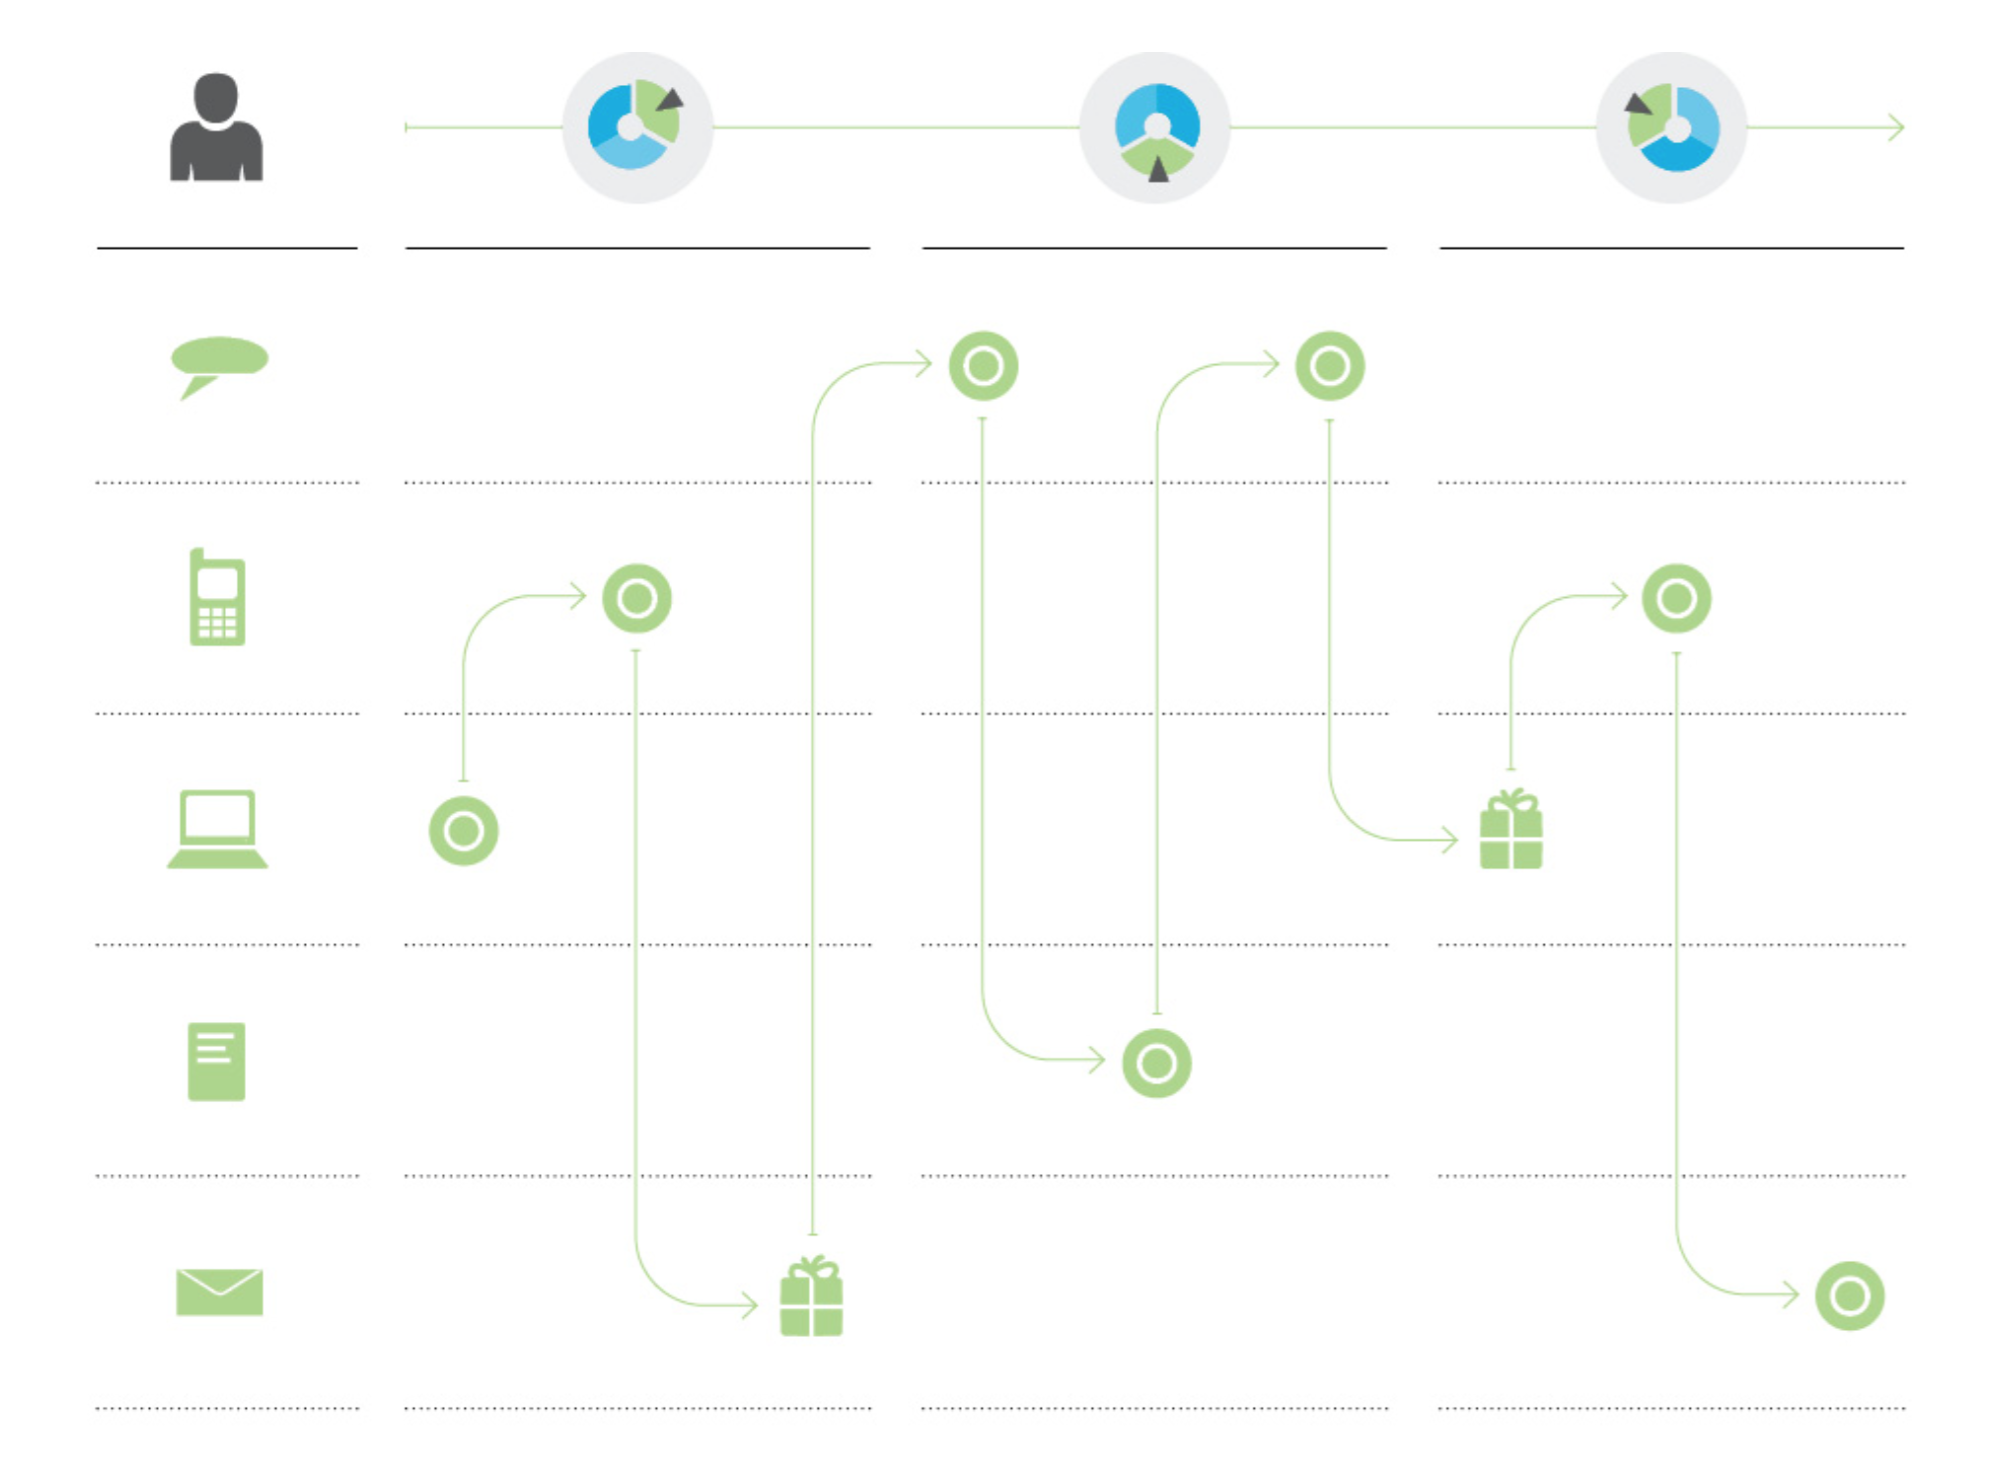
\includegraphics[width=0.7\textwidth]{analysis/cjmExample.png}
    \caption{General example of a customer service map. The map is divided by channel (could also be by a persona) and time (in this case before, during and after using a service).}
    \label{fig:cjmExample}
\end{figure}

The customer journey map is beneficial both for understanding a user's touchpoints with a service, and also for collecting and analysing stories which explain why the journeys happened as they did \citep{stickdorn}.

\subsubsection{Sprint Backlog}
During product development, to do a sprint backlog is a kind of data analysis. When a high altitude of ideas and feedback has been gathered, a sprint backlog is a list sorted with the most important and urgent items on top.

To work through ideas in a structured way, requests are categorized into what is called "stories". A good story answers "As a [user type] I want to be able to do [feature] so that [benefit]". Each story can then be broken down into todos ("What needs to be done in order to satisfy the story?"). During the sprint planning, the most important stories and todos are identified. By analysing and then working on the most prioritized story and todo, you ensure that you are always working on what is most important for the success of the project.

At the end of an iteration, as much as possible of the sprint backlog has been taken from "Not done" to "Done". The things not done, can either be moved into a product backlog (to later be added into an upcoming sprint backlog) or removed (they were not important enough).

\subsubsection{Sprint Demo}
A sprint demo is an effective way to analyse the product created after an iteration, from the perspective of the users and the stakeholders. \cite{kniberg} says that a well executed sprint demo attracts vital feedback from stakeholders, and ensures that todos are 100\% done. A sprint demo does not need to be complicated: the product is shown and tested with users and stakeholders, getting feedback for the next iteration. But without it, it would not be possible to know if the work done has satisfied the needs of the end users, or what the stakeholders thinks is important for future work.

\subsubsection{Quantitative Data}
Below, methods for analysing collected quantitative data are presented. The first method is correlation, but if multiple variables needs to taken into account, logistical regression can be used. As both of these are statistical tools, they rely on statistical significance in order to be trustworthy. In small-scale app tests, such amounts of data might not be sufficient.

To find trends or oddities in a small data set, visualization techniques to discover the data by hand might be more beneficial. To enable a visualization, the data needs to be collected, enhanced, mapped and rendered. When rendered, a suitable rendering of a multiple-variable data set might be parallel coordinates, which shows correlations graphically, and can be made filterable by user interaction.

\subsubsection{Calculating Correlation in Google Sheets and R}

The process is to calculate and compare means on a "control"  with a response variable.

It is clear that analysis in Google Sheets can only go so far. It can be greatly helpful to sort by multiple columns (e.g. first by Manual?, then by School level, then by Quiz 3). However, it takes a long time to filter the data on multiple parameters, and the work easily becomes tedious. For some applications, it may not be viable to discover the data using this approach.

In Google Sheets, color scale can be used to give different column values different colors, see figure \ref{analysFarg4}. It is still hard to compare all of the axises towards all the axises, and it is not a scientific approach.

Even in R, it is cumbersome to do statistically with all of the axises against all the axises. It is however possible to in both Google Sheets as well as the R programming language. Psuedo-code in R would be:

\begin{verbatim}
x1 = c(1,2,3,1,5,6)
x2 = c(2,3,4,NA,6,7)
cor(x = x1, y = x2)
cor.test(x1,x2)
\end{verbatim}

In R programming language there are more powerful tools for visualizing the correlation, e.g. using a "Correlation Heatmap", see figure \ref{fig:corrHeatmap}. Psuedo-code in R would be:

\begin{verbatim}
random_matrix <- matrix(rnorm(100), nrow = 10, ncol = 10)
random_matrix[1,1] <- NA
colnames(random_matrix) <- paste("V",1:10)
cor_mat <- cor(random_matrix)
heatmap(cor_mat, keep.dendro = FALSE)
\end{verbatim}

\begin{figure}[h]
    \centering
    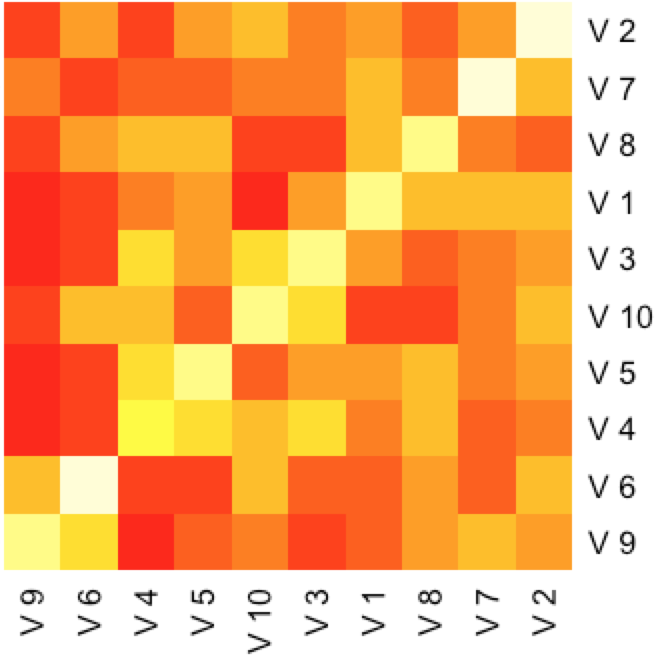
\includegraphics[width=0.7\textwidth]{analysis/rStatisticalAnalysis.png}
    \caption{Heatmap showing correlation, axis against axis, using example data. The more red a segment is, the bigger is the correlation between those two axises. You can see that in this example, there is a big correlation between for example V4 and V9.}
    \label{fig:corrHeatmap}
\end{figure}

\subsubsection{Calculating Logistic Regression in R}

A limitation with correlation is that only two dimensions can be compared with each other at the same time. What if we want to find a correlation between quiz score and gender \textit{and} age?

To do this, Logistic Regression is helpful if our response variable can be a logistical dimension (e.g. women or male, used manual or not), while linear regression needs to be used if it is a linear or nominal scale (e.g. age and city respectively).

In either case, the first step is to determine a response variable: the variable to compare against, e.g. is there a difference between men and women? In this case, it needs to be a quantitative measure of: "Have you learned anything?".

If one more variable is added, e.g. also adding if a manual was used, this is called the "control". It is possible to add as many controls as possible.

If linear regression, then it is needed to determine a quantitative measure of ("How much have you learned?").

In Google Sheets, this is not effective to do. R, however, is a very suitable tool. First, the data is loaded, e.g. as a CSV file. Then, we tell R which the N/A values are, e.g. "N/A" or "Vet ej". We use this to filter the data. Then, each column we want to use is converted into a factor.

When factors, a model can be created, e.g. using the General Linear Model. A different family can be selected, e.g. binomial.

Then it is possible for R to show this data, showing the coefficient, the Pr value, and others. See code below.

\begin{verbatim}
mydata <- read.csv("Development/R/quizResults.csv", na.strings = c("N/A", "Vet ej"))

mydata$y = ifelse(test = is.na(mydata$Quiz.9..y.n.1st),  yes = 0, no = 1)

mydata$y <- as.factor(mydata$y)
mydata$Help <- as.factor(mydata$Help)
mydata$Sex <- as.factor(mydata$Sex)

mymodel <- glm(formula = y ~ Pre.test.score + Sex, data = mydata, family = 'binomial')

summary(mymodel)

plot()
\end{verbatim}

For analysis, looking at the summary, coefficient (e.g. -1.0704) shows either a negative or positive correlation (in this case -7\%) for what to compare with as a response variable.

To be significantly significant, a common measure is that the Pr value ("the p-value") needs to be higher than 0.05. If the p-value is higher than 0.05, meaning it is significant with a 95\% probability.

\subsubsection{Visualizing and Analysing Multi-Variable Data with Parallel Coordinates}

\cite{timo-ropinski-liu} describes the "visualization pipeline", generating an image from data:

\begin{enumerate}
\item Data acquisition ($\,\to\,$data are given)
\item Data enhancement ($\,\to\,$ data are processed)
\item Visualization mapping ($\,\to\,$ data are mapped to for example a geometry)
\item Rendering ($\,\to\,$ images generated)
\end{enumerate}

% Timo Ropinski, Scientific Visualization Group, Linköping University, TNM067 - Scientific Visualization, 9/12/2014)
% https://drive.google.com/drive/u/0/folders/0BzlK1PD8EE75bHIxcXRQNWpRMm8

Data acquisition presents how data was acquired. Data enhancement explains how the data was processed. Visualization mapping is the process of mapping data to e.g. a geometry. Finally, rendering allows images to be generated, presented in 2D. This image can then be analysed.

What rendering to do, depends on the situation. In a multiple-variable data set, parallel coordinates is often a suitable visualization, especially if there is a lot of data for each axis.

Parallel coordinates allows you to see relationships and trends between dimensions. They can be seen by a positive or negative relationship (correlation or invert), or no relationship at all (random) \cite{une-terre}.


\section{Setting and research context}
Uganda (Kampala, Tororo) and Zambia (Kabwe).

The biggest challenge with regards to time constraints and cultural differences is that it is difficult to understand the audience.

It led to me choosing to spend 3 months in Uganda, because the client and academy is there, and start the design process when I'm there. It also led me to wanting to apply service design.

By being in Uganda and applying service design, I will come closer to the client and coaches.

The internet is worse, especially outside Kampala (I will not be able to access 4G, and prices are high).

Working mainly from Kampala, because that is where YoungDrive is situated, means that there is still a long distance to the coaches in Tororo, which is located near the Kenyan border.

\section{Subjects (Participants) \& Stakeholders}

Lorum ipsum.

Participant manual and Coach guide

\section{Study Design and Data Collection}

  As a computer expert with social skills needing to design and develop an app for a unfamiliar cultural and socio-economic context, it was needed to quickly become a good designer.

  The technical aspect of the project was but one. It was needed to learn how to develop hybrid apps in JavaScript that worked offline, and had an online back-end. However, those are merely the technical demands.

  It was needed to quickly become a good designer, not mainly from a perspective of graphic design or interaction design, but \textit{how} to explore, design, and implements what the user needs from the requirements "fun, user friendly, and good for learning". The approach used to learn design from these perspective was to read extensive literature, consult a diverse set of experts, and be humble and curious in interactions with the end-users and stakeholders.

  In the following section, the creation and implementation for a suitable design process is described, together with the study design and data analysis for each iteration of the project.

%Har gått igenom planeringsrapporten lite noggrannare idag och ser två saker som vi kanske ska borde fånga upp under arbetets gång.

% Under 2 Purpose står det ett upplevelsemål från Young Drive. Bör vi mäta detta upplevelsemål om det stämmer med deltagarnas faktiska upplevelse, d v s ska vi försöka få in det under 3 Research Questions?

% På våra avstämningsmöten borde vi också följa upp dina Research Questions så att kundinteraktionerna och servicedesignmetoden tyligt leder dig framåt mot dessa mål.
%* Reflektioner på vilka designprinciper som bör väljas? (utifrån kundinteraktioner)
%* Reflektioner angående tekniska begränsningar?
%* Reflektioner på processen?

\subsubsection{Creation of Design Process}
As there was a unfamiliar target group - mostly young Ugandians with little or no experience of smartphones - service design thinking would benefit true understanding of cultural context and in-depth empathy for the end users.

Tools and methodology in service design were chosen with the help of Expedition Mondial in Stockholm, who provided education and coaching.

At the same time, the end result would be a digital artefact (an app), which is not common in service design.

While this product could be though of as a service, the tools and methodology would benefit to borrow from Agile methodology and Interaction design.

I'm the computer expert kind of designer \cite{lowgren}, adjusted to agile methodology and interaction design, but aspiring to be a socio-technical expert. Expedition Mondial are experienced with service design, aspiring to be more of computer experts.

This led to the joined development of a Digital Service Design method, co-created by the both.

%Expedition Mondial helped with a method for creating a MVP of the digital support for the coaches, so that the app was developed from the perspective of the end users and the education and a "learning by doing" mentality.

%The suggested design process was designed with them after a start-up meeting on Skype, and an education day in Stockholm. During that day a crash course in service design was given, then creating a common plan for the future work based on my needs (see Appendix: Original Time Plan \todo{Add reference}). They also recommended service design literature. These were the methods chosen in each iteration.

The result is that the design and development phase in Uganda is an iterative process with the human in focus. The process is built on top of service design process and methodology, while in-line with digital design practices.

\subsubsection{Implementation of Design Process}
There were four iterations. The first iteration follows Service Design, not starting the app development, while the other three follows the new methodology, Digital Service Design.

In iteration 1, there is a very broad scope, without digital focus, where iteration 2, 3 and 4 introduces and narrows down the project into a digital solution.

Expedition Mondial gave support in each iteration, helping with refinements of each iteration as learnings happened along the way, and they were able to educate me during the different stages with methodologies whenever necessary.


\subsection{Iteration 1: Uganda Coach Visit}

% How was this iteration designed?

Following the service design sequencing, the first iteration had a very broad scope and truly is a service design iteration: "From your perspective, what is it like being a coach?". \footnote{A coach meaning either a Community Based Trainer (carrying out all the trainings), or a YoungDrive coach, depending on who was asked the question.} \cite{lowgren} was used how to start the project, meaning that the purpose was to get a preliminary understanding of all important aspects, and build relationships with all stakeholders.

%The project started with a startup meeting with Shifteh from Plan International in Kampala, together with Iliana. From there, I did research and met with Grameen Foundation and Designers Without Borders, before going to Tororo to research "What's it like being a YoungDrive coach?", and determining how advanced an app could be to solve challenges that the coaches face.

Insights depended heavily on interviews with all the stakeholders  (2 with Plan International, 3 with YoungDrive), and local experts (1 visit each at Grameen Foundation and Designers without Borders, 1 workshop with Mango Tree), since no Interactions with users had been made yet. Also, knowledge and connections were made with the Kampala tech scene as much as possible, from the new home and office in Kampala, working at the tech hub and co-working space Hive Colab.

Ideation were about creating a questionnaire guide for the interviews, a co-creation workshop using "Customer Journey Map", and identifying how the app test should be designed to test their existing knowledge (and be informed of the design preferences of the YoungDrive app).

Trigger material was the finished questionnaire guide (constructed with Expedition Mondial) a written plan for the co-creation workshop ("A day as a coach"), and a written plan for testing the quiz app Quizoid and the language learning app Duolingo, and a schedule for the interactions.

The interactions were focused on design ethnology, getting to know and learn from people in a different culture, namely the coaches. The focus was on the their needs, motivations, and context.

To accomplish these, four days were spent in Tororo, with one day of travel. There were four face-to-face-interviews,
one meeting with Plan, one meeting with the local partners, two workshops, one coach stay-over, and two youth session visits (one of the youth sessions are observable via figure \ref{fig:youthsession}.

\begin{figure}[h]
    \centering
    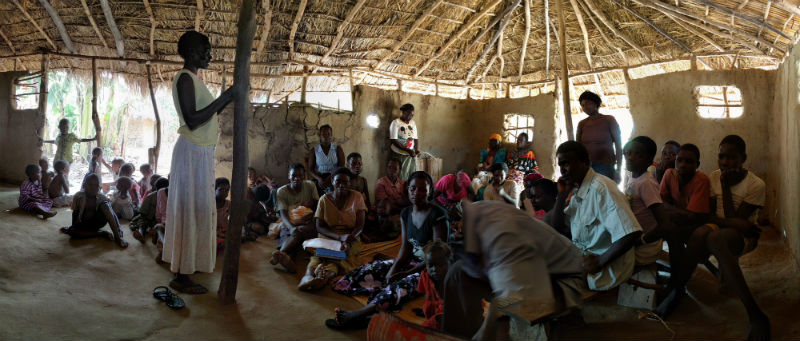
\includegraphics[width=0.7\textwidth]{youthsessionSmall.jpg}
    \caption{Photo from the location where one of the youth sessions were held. Here, a CBT in Tororo teaches youth in basic sales and marketing.}
    \label{fig:youthsession}
\end{figure}


\subsection{Iteration 2}

This time, the iteration has a more detailed scope, with a hypothesis on what needs the app should meet in the end, and create lo-fi and hi-fi trigger material to meet those needs.

A co-creation workshop started the interactions, followed by repeated app tests at minimum one session per day, always followed by a feedback round, so the app and the tomorrow's question set creation could be improved for the next day. At the end of the week, there was a co-refinement workshop of the current hi-fi material, and also lo-fi material for the new version of the app.

\subsubsection*{Creation of questions}
Project leader Josefina in Zambia refined Iliana's first question sets, prepared for my visit in Zambia. Josefina created question sets with Bloom at the back of her head, also taking into account the structure and the order of the coach manuals, what it means being a coach within the topic, and lastly scenarios.

\subsubsection{Trigger material used}
A hi-fi trigger material was done, a very basic quiz app, keeping it as simple as possible (see Application Implementation, Iteration 2). All of the devices (tablets and smartphones) that I had available were brought to Zambia.

I added Josefina's questions to the app, and installed the app to all of the devices. This process was repeated for all the days, Sunday-Friday.

\subsubsection{Design workshop \#1 in Zambia}
The coach training started with me having a design workshop with the coaches, not showing them the app that I had created. The co-creation workshop was made to identify important functionality in the minds of the coaches.

\begin{enumerate}
\item Since the knowledge about smartphones and apps were low, I started by introducing these topics.
\item All were familiar with Facebook, so thus I showed the Facebook app. Me wanting to know what the app would look like if the coaches would have designed the app, I first needed to train them how to design an app via drawing wireframes.
\item Using postits, they started with during limited time drawing the start view from the Facebook app.
\item Then, they were asked to draw what they thought happened on the friend icon click, drawing the view on another postit.
\item Then, the mission of the YoungDrive app was described. They were then divided into two teams, having limited time to draw the best imaginable YoungDrive coach quiz app they could. First, they designed the app from the top of their heads. They then pitched their results to each other.
\item On the next iteration, they were to suggest and design improvements how the app should be designed to improve learning, not only assessment. They then again pitched their results to each other.
\end{enumerate}

\subsubsection{Assessment via quiz}
At the end of each day, the app was used to test the coaches' knowledge. Each coach got either a smartphone, tablet or computer. The coach first took the quiz for the most recent session, and could then choose what to do next.

As there were no back-end developed, Josefina by hand documented the scores of each coach, writing the name of the coach, the session, number of correct answers, and what questions had been answered wrong.

Josefina then, when planning the next day, looked at the statistics, looking for trends that would inform the sessions for the following day.

She also evaluated the quality of the questions, before creating the new question sets for the next day.

\subsubsection{Experimenting with quiz before or after the session}
Since the coaches appreciated the app so much, we felt tempted to try what would happen with fun and learning if we tried using the app \textit{before} a session instead of only after. During the rest of the week, we continued, finally finding preferences and tendencies from the coaches, via observation, interviews, and survey.

\subsubsection{Experimenting with design of questions}
During the week, extra tests were done to test the following:

\begin{itemize}
\item Number of questions per quiz
\item Single-answer questions or multiple-answer questions
\item Framing of questions
\item Challenge level of questions
\item Determining what made a question hard
\end{itemize}

\subsubsection{Interviews with Josefina}
At the end of each day, an evaluation interview was held with Josefina. At the end of the week, a final interview was held.

At the end of Day 5, Josefina and I discussed what it would look like to not record the answers manually, but pushing the results online. A co-creation workshop was held, where she drew an Educator Dashboard.


\subsection{Iteration 3}

Because of the many research and functionality needs, the study design of Iteration 3 became very important. A lot of development and ideation needed to be done.

\subsubsection{Iteration 3: Purpose}
Iteration 3 had an even more detailed scope. Since the app now succeeds with the first use case, the coach training, now the focus could be on "learning at distance".

\subsubsection{Pedagogical model}
It was chosen that "Are you sure?" + Improve would be included in the hi-fi material, a flip-card approach would be tested as a lo-fi material, and to "record answer via voice" could only be presented as an idea during a field interview (experts said there would be usability issues, and the 1st-time smartphone user agreed). The Gold/Silver/Bronze method was included into the hi-fi material.

\subsubsection{Test on a Kampala entrepreneurship student}
Also, instead of only testing the app in Tororo, a test was held in Kampala, to get feedback from an entrepreneurship student.

\subsubsection{Test in Tororo}
As Plan International staff are not allowed to support visiting coaches in the field during local elections, the co-project leaders in Tororo were consulted to carry out the field trips, so that it was still possible to attend the youth group meetings.

For the interactions, a big app test was held, a group interview was held, and then they were divided into co-creation workshop groups, with a presentation in the end.

%Before the workshop, the wished functionality and goals were well formulated. It was also discussed beforehand how to best design the workshop, together with Linköping University and Expedition Mondial.

There was another partner meeting, with Plan International and Community Vision present. There was an app test with all of the coaches, "Testing the YoungDrive coach app", followed up by splitting into six workshop groups based on solving different problems discovered during the test.

The following day, there were three field visits to CBTs, observing how they prepared themselves for a youth session, and then testing the app for assessing and becoming prepared for a session.

After the app tests, it was tested with a lo-fi prototype that the coach thinks aloud about the question, \textit{before} receiving the multiple-choice answers. This approach proved to be great for learning, and could be a great addition to the hi-fi material. Interestingly, this test was done as a live quiz, and if the interviewee could not answer the question directly, the audience were asked and tested if they knew the answer (raised hands), and if nobody knew the answer, it was tested which of the multiple-choice alternatives they found most likely.

During the afternoon, we divided into 5 groups focusing on improving the app experience for the coaches.

On Wednesday, the coaches from the field visits were gathered for a workshop. The purpose was to see how they acted when given the challenge: "Get 100\% correct answers in one go, on the hardest quiz". A co-creation workshop ("Educator Dashboard") was held in parallel, with 3 CBTs and 1 project leader respectively.


\subsection{Iteration 4: Uganda Summative Test}

The focus of iteration 4 was a summative test. First, a pre-test was carried out in paper, including questions about the coach and an entrepreneurship quiz, based on a well-known study \citep{general-entrepreneurship-quiz}, see Appendix \ref{cha:pre-test}. During the test, this was the first time that the app could send data to the server. Data was sent whenever a quiz was started, and whenever a quiz was finished. The group was divided into two, the ones who brought manuals and they who did not. Those that had brought manuals, could use these with the app, see figure \ref{fig:appevaluation}.

\begin{figure}[h]
    \centering
    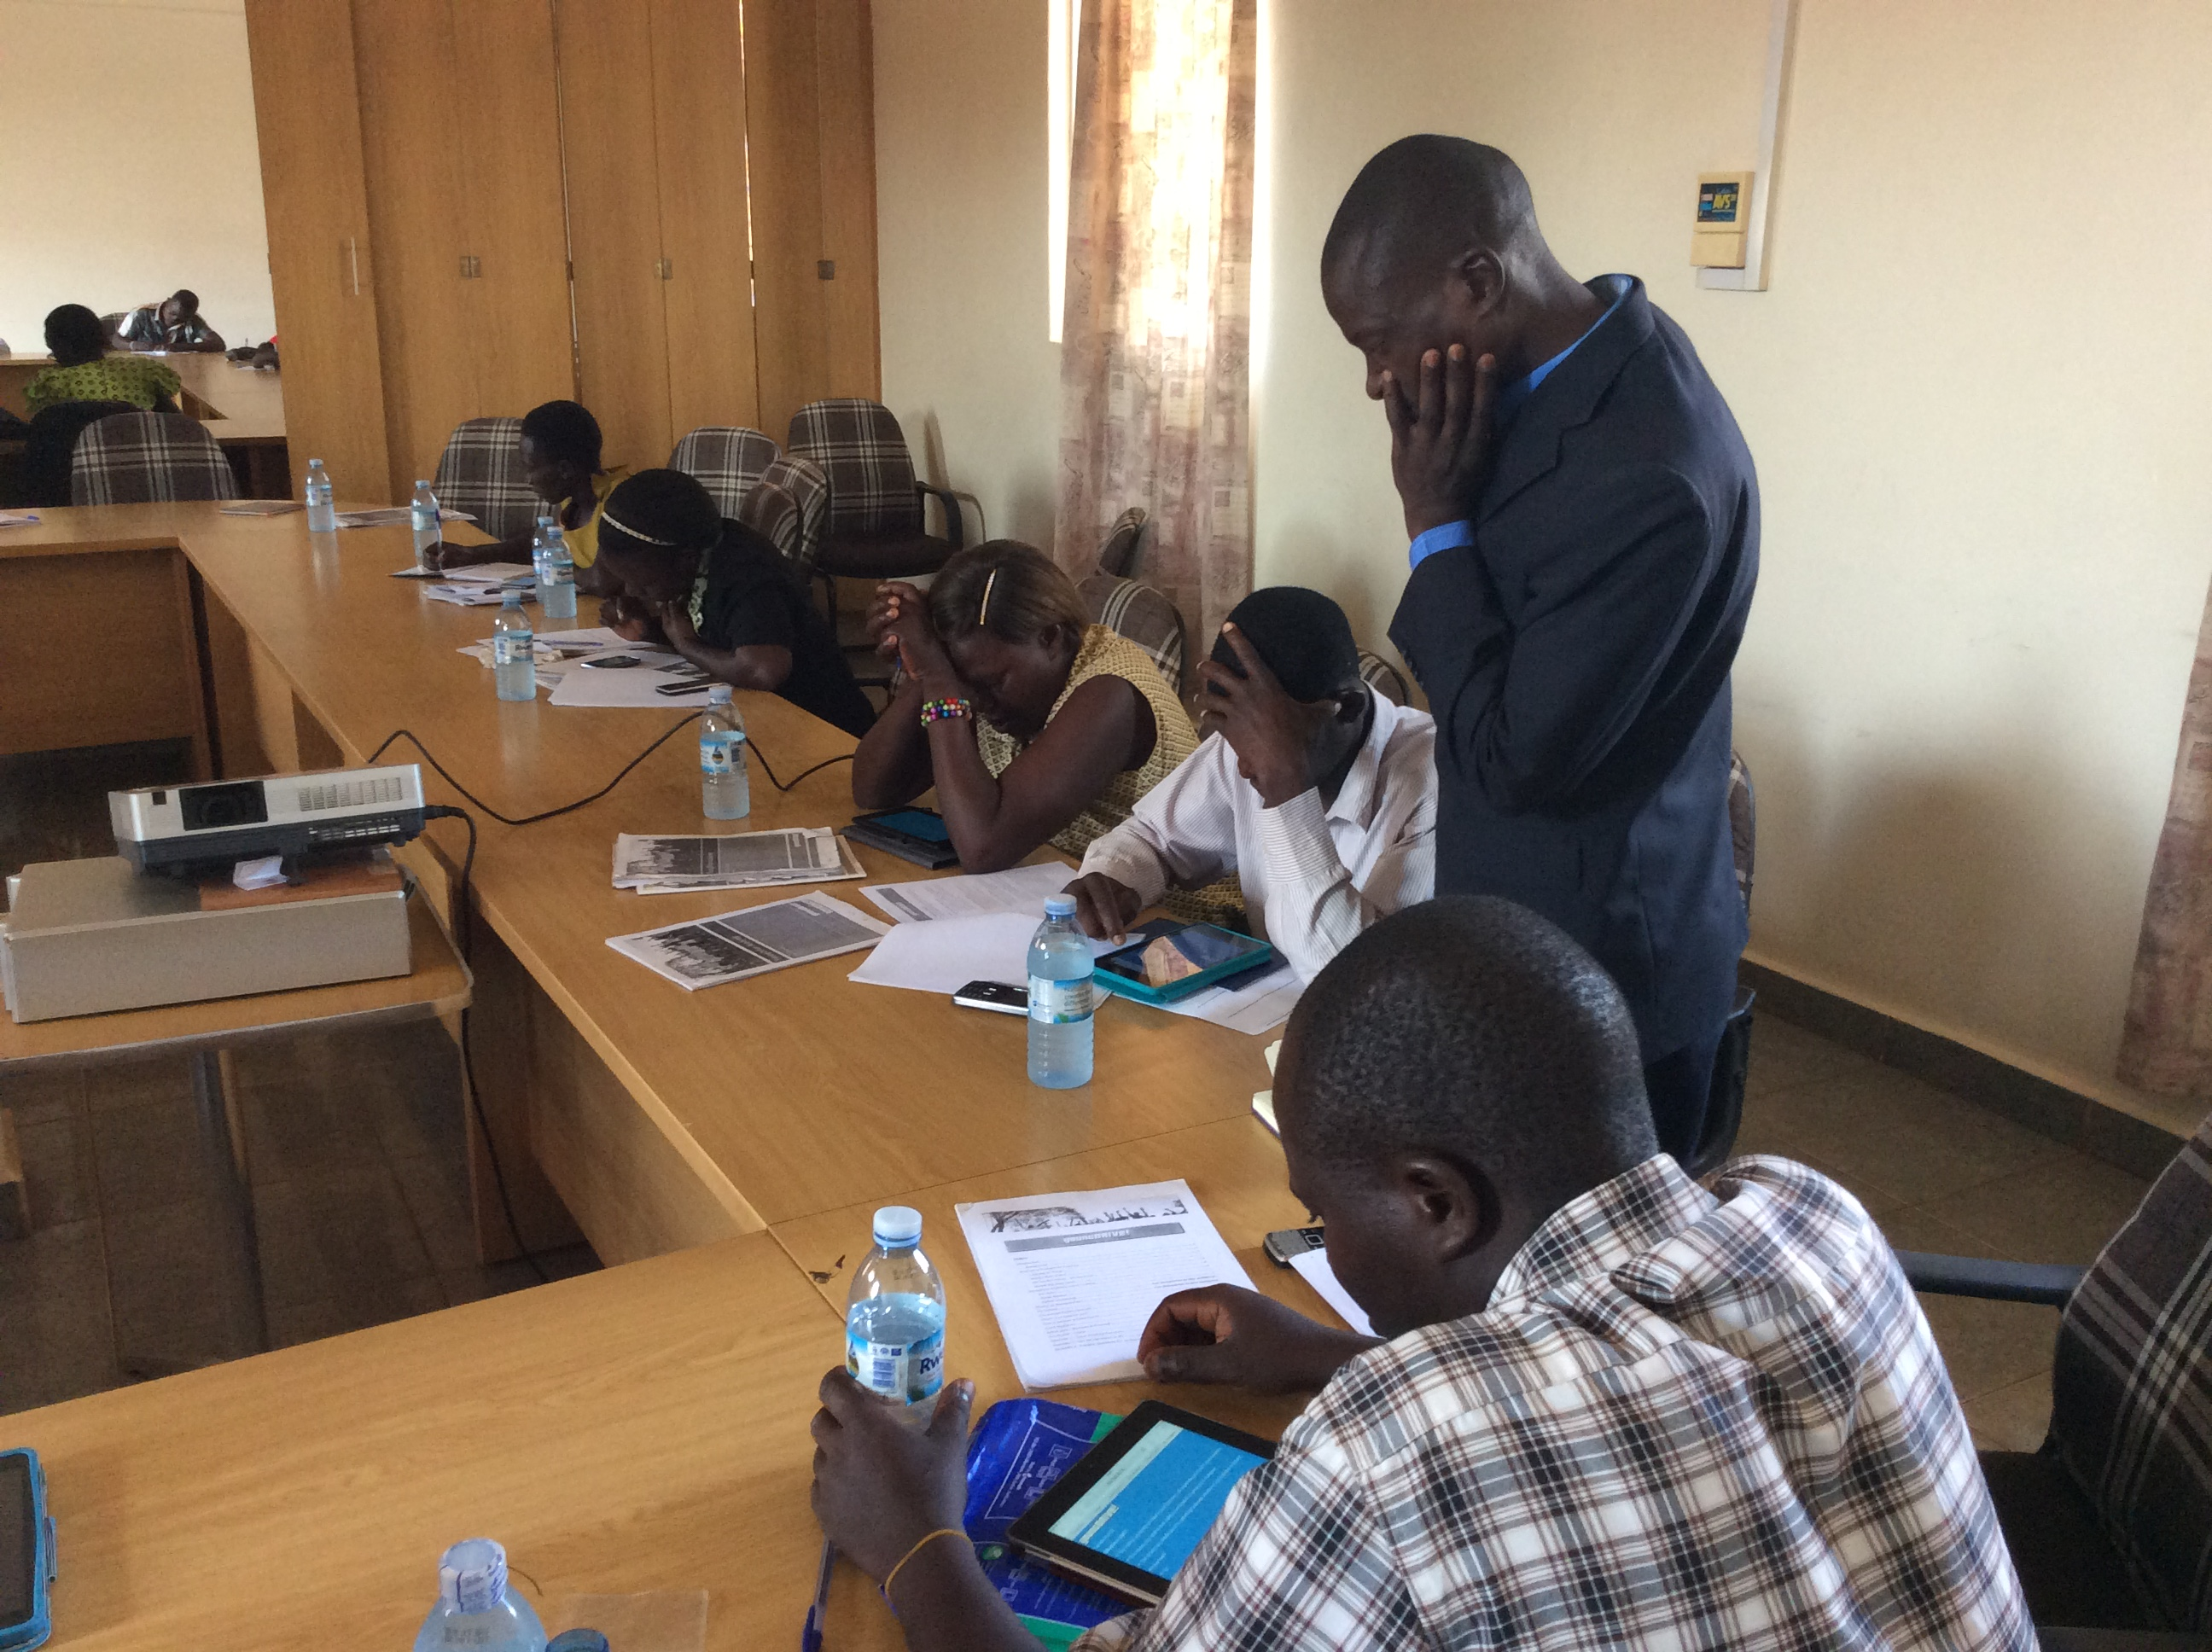
\includegraphics[width=0.7\textwidth]{appevaluation.jpg}
    \caption{Coaches answering the app questions for topic quiz 3 on Financial Literacy, and the coach guide quiz 9 on Action Plan.}
    \label{fig:appevaluation}
\end{figure}

After the test, every coach was divided into one or three groups, on random. In these groups, they were asked:

\begin{enumerate}
\item Why do you think you were correct or incorrect?
\item Do they like the app?
\item Are you stimulated by the app?
\item What did you like?
\item What did you not like?
\item When do you want to use the app?
\item When are you not able to use the app?
\end{enumerate}

To analyse the paper-submitted data, all of this was combined first into a Google Spreadsheet (the app results were also recorded in paper, but only as a backup). Data collection was done by the app itself, which pushes data to server whenever online (it saves quiz start, and quiz finish).

%The next day, a small app evaluation and co-creation workshop was held for the Educator Dashboard, and the final version of the app. Also, a test was done with the Plan Tororo staff.

%Back in Kampala, a presentation was held with Plan International. Back in Sweden, a presentation was held with the YoungDrive Strategic Management Team.



% Application implementation
\section{Application Implementation}

In this section, the prerequisites for the app is described, from the perspective of the user, stakeholders, and the developer.

\subsection{User Needs}

The technical constraints for the project, would need to affect the technologies used, if the project would be user-centered.

On the client side, the app would need to be mobile and web based, consider non-access to internet, and not use a lot of battery, to work for the coaches of YoungDrive.

That the app should be simple to use in this cultural setting leaded to design constraints and needs for evaluation.

\subsection{Stakeholder Meeds}

As the project was only three months, and the first month would be without digital development, time constraints were massive. However, to be able to answer research question \#2, evaluation needed to be done via data collection.

If no evaluation, there would be no need to write code, instead working with a lo-fi prototype using pure design tools. Now, a data-driven approach was needed to measure, and therefore an app needed to be developed.

On the server side, a database and API would be needed, to pull data from the database and push data from the client. Since internet was not always available, the client must be smart in its usage of pushing and pulling data. This would need to be investigated further into the project.

\subsection{Devices to be Used}
As most of the coaches did not have smartphones or tablets, four smartphones (3 Android, 1 iOS) and ten tablets (3 Android, 7 iOS) were brought from Sweden. All of these devices had a web browser and access to an app store. These were either donated, borrowed or bought devices. During the user tests, also using a laptop would be tested.

%\subsection{App/Web Development}
%Early in the project, it was thought that existing tools could be used, instead of building the app from scratch. E.g. using existing tools like Knowly or Typeform\footnote{examples include https://showroom.typeform.com/to/ggBJPd and https://showroom.typeform.com/report/njdbt5/dIzi} during the first iterations for understanding users, and during development e.g. the Typeform API (http://typeform.io/). The Typeform API allows developers to create surveys from within their own applications or systems.

\subsection{Choosing Frameworks for Creating the App}

A JavaScript framework helps and speeds up the creation of building web apps. In the start of the project, Meteor \citep{meteor} and Ionic Framework \citep{ionic} were both tested and compared with each other. It was decided that Meteor was the best way forward, partly because it would allow the app to be accessible on the web as well. %\todo{Add from mindmap}

React \citep{react} (a JavaScript library for building user interfaces) was chosen as the front-end framework, having integration with Meteor and being relatively easy to learn and fast for development.


\subsection{Iteration \#2}
Here, the work and result from iteration \#2 is presented.

\subsubsection{Staging environment using Heroku}
Needed when the Meteor free tier was removed. Connected to deploy from GitHub branches automatically. Could have benefitted from CI, passing tests before ready for production. Solved this by having a stage environment (since April 19th) where stage is YoungDrive-beta (branch Iteration 4), and YoungDrive is master.



For iteration 3, as components grew, there was a need for a client-side router. The Meteor plugin Flow Router was used, as it was very popular with good integrations.

For iteration 3, there was also a need to store data per individual, partly because the feature was prioritized from YoungDrive, but also because of the purpose of data collection. In order to store data per individual, a database and login would be needed. Because of technical difficulties, login and automatic data collection was not implemented until iteration 4, which can be read more about in the Discussion in \ref{backwards-capability}.

\subsection{Login}
To record data per user, would require login. This would be a usability issue for most problems, being 1st-time smartphone users. They need to find it intuitive, user-friendly, and be able to remember the password in the future. A lot of different suggestions were through the ideation phase.

The simplest login possible was chosen, after evaluation and discussion with experts: a 3-digit code, which was to be given to each coach during the test.

%Jag pratade med flera om detta, Expedition Mondial och Grameen. Från EM lärde jag mig att de trodde min idé med en färdiggjort lista med coachernas namn (vi vet ju vilka som är i Tororo) skulle fungera, och från Grameen fick jag höra om dera erfarenhet att de validerat använda samma approach, med en PIN (längre än 4 siffror dock), men att de inte nailat konceptet ännu, och att de också itererar på sin approach för nästa uppdatering av LedgerLink.

Meteor had limitations with their auto-login module, which is very fast to implement. It forces username and password, and instead I wrote the login myself. This was

To summarize, the front-end was not problematic, however, implementing server-client communication so that it worked online and offline, was.

%Tyvärr har också Meteor begränsningar med deras auto-login-modul. Den tvingar både användarnamn och lösenord, och har automatiskt registrering. Går det att stänga av? Jag kan skapa användare och lösenord åt alla, och funderade på hur jag skulle generera lösenord. Ett förslag blev att bara registrera deras förnamn, och sedan skapa lösenordet baserat på T9 med de 6 första bokstäverna utan att berätta det för dem. Sedan tänkte jag på det kulturella, att det kan vara oartigt med förnamn, och bestämde mig för efternamn istället. Hela namnet skulle bli för långt och krångligt.

%Helst skulle jag behöva gå runt Meteors standard-inloggning, och istället ha en enkel login-rullista som den ovan beskrivet, istället för att använda deras standard-lösning.

\subsubsection{Online and offline database}
If data was to be sent from the client to the server, there needs to be a database with Meteor Collections. An example app was made first, only using Meteor Collections. Meteor's use of Distributed Data Protocol (DDP), made app pushes feel immediate, even though data was not sent until there was Internet access.

However, it was found out that if it took more than 15 minutes to get online, the push would be aborted. For users that are seldom online, this would not be viable.

An offline database was needed, and the plugin GroundDB was implemented. As it was cumbersome to get right, pushing the data whenever online, and hard to test (needed to wait 15 minutes each time), this was not ready for the interactions until Iteration 4. As a consequence, until iteration 4 of the app, no results were saved online via the app whatsoever.



For iteration \#4, data collection was done by the app itself, which pushes data to server whenever online (it saves quiz start, and quiz finish). The server receives JSON data from the client, stored in the MongoDB database hosted on Heroku. Each data point is saved in a database called Results, with the signed in user (from the Users database). In the database, there are collections for Users, Quiz Lists, and Quiz Results.




\section{Data Analysis Theory}

%\todo{Lägg till overall data table}

%Methods to choose from for analysing (i.e. what I did during the interactions, to test and analyze my app)

%Partly data collection done via app, but also all the observations

The results from each iteration needed to be analysed, using the methods outlined in section \ref{sec:data-analysis}. Depending on the kind of activity and results gathered, different data is collected.

For qualitative methods, the output is almost always observation notes, which are then concluded into insights. These insights, can then sometimes be used in the below analysis methods.

For quantitative data, the output is almost always quiz results or data about the coaches. Before analysis, how this data has been processed is clearly described in chapter \ref{sec:data-analysis}.

Below, an overview of which data analysis method was used for what data is presented. The tools and iteration the tool was used in, is outlined below as a summary:

Qualitative data analysis:
\begin{enumerate}
\item Need groups and Personas (\#1)
\item Customer Journey Map (\#1)
\item Sprint backlog (\#1, \#2, \#3, \#4)
\item Sprint demo (\#1, \#2, \#3, \#4)
\end{enumerate}

Quantitative data analysis:
\begin{enumerate}
\item Correlation in Google Sheets (\#2, \#3, \#4)
\item Correlation in R (\#4)
\item Logistical regression in R (\#4)
\item Parallel coordinates visualisation (\#4)
\end{enumerate}

\subsection{Iteration 1: Uganda Coach Visit}

In iteration 1, the following activities were carried out and then analysed:

\begin{itemize}
\item Stakeholder interview (for Need groups)
\item Coach interview and field visit (for Need groups)
\item Workshop (for Customer Journey Map)
\item Smartphone test (for Need groups)
\end{itemize}

\subsection{Iteration 2: Zambia Coach Training}

In iteration 2, the following activities were carried out and then analysed:

\begin{itemize}
\item App test observations (for Sprint backlog)
\item Quiz results (for Sprint demo)
\item App design workshop: use case 1 (for Sprint backlog)
\item App design workshop: use case 2 (for Need groups)
\end{itemize}

\subsection{Iteration 3: Uganda Formative Test}

In iteration 3, the following activities were carried out and then analysed:

\begin{itemize}
\item App test observations (for Sprint backlog)
\item Service Mini-Sprint - 5 workshops (for Sprint backlog)
\item Field visits (for Sprint demo)
\item Small formative app test (for Sprint backlog)
\item Big formative app test (for Sprint demo)
\end{itemize}

\subsection{Iteration 4: Uganda Summative Test}

In iteration 4, the following activities were carried out and then analysed:

\begin{itemize}
\item Big summative app test (for Sprint demo and quantitative analysis)
\end{itemize}

Data analysis of quiz results were done first by a general overview in Google Sheets, by statistical analysis in R, and by a parallel coordinates visualization. The process to do this, is described below.

\subsection{Analysis Implementation of Quiz Results and Pre-Data}

In this section, the steps needed to analyse the quantitative data is explained in detail, so that others can use a similar approach. In this example, quiz results are from iteration 4, but a similar approach has been taken with the manually recorded quiz results from iteration 2-3 as well.

Data analysis of quiz results was done first by a general overview in Google Sheets, by statistical analysis in R, and by a parallel coordinates visualization. The process to do this is described below.

\subsubsection{Step 1: Data Acquisition from Server}

It was desired to store the data in Google Sheets, thus it was necessary to collect the MongoDB database content, and convert JSON format into a Google Sheets-readable format, like CSV. Multiple approaches were tried, and the Google Chrome extension called Magic Json \citep{agaze} was the one that worked without problems.

\subsubsection{Step 2: Data Acquisition from Pre-Study}

The Pre-study data acquisition was done by instead of looking at the paper-submitted pre-study evaluation forms, using the data processed into Google Sheets.

\subsubsection{Step 3: Data Enhancement of Server Results}

This section presents how data from the server was processed, to enable visualization mapping. To make the data easier to work with, the columns were reordered, and made sortable and filterable. Some columns were given conditional formatting, so it would be easier to spot irregularities, see figure \ref{fig:resultsColored}. After this, some observations could be made.

\begin{figure}[h]
    \centering
    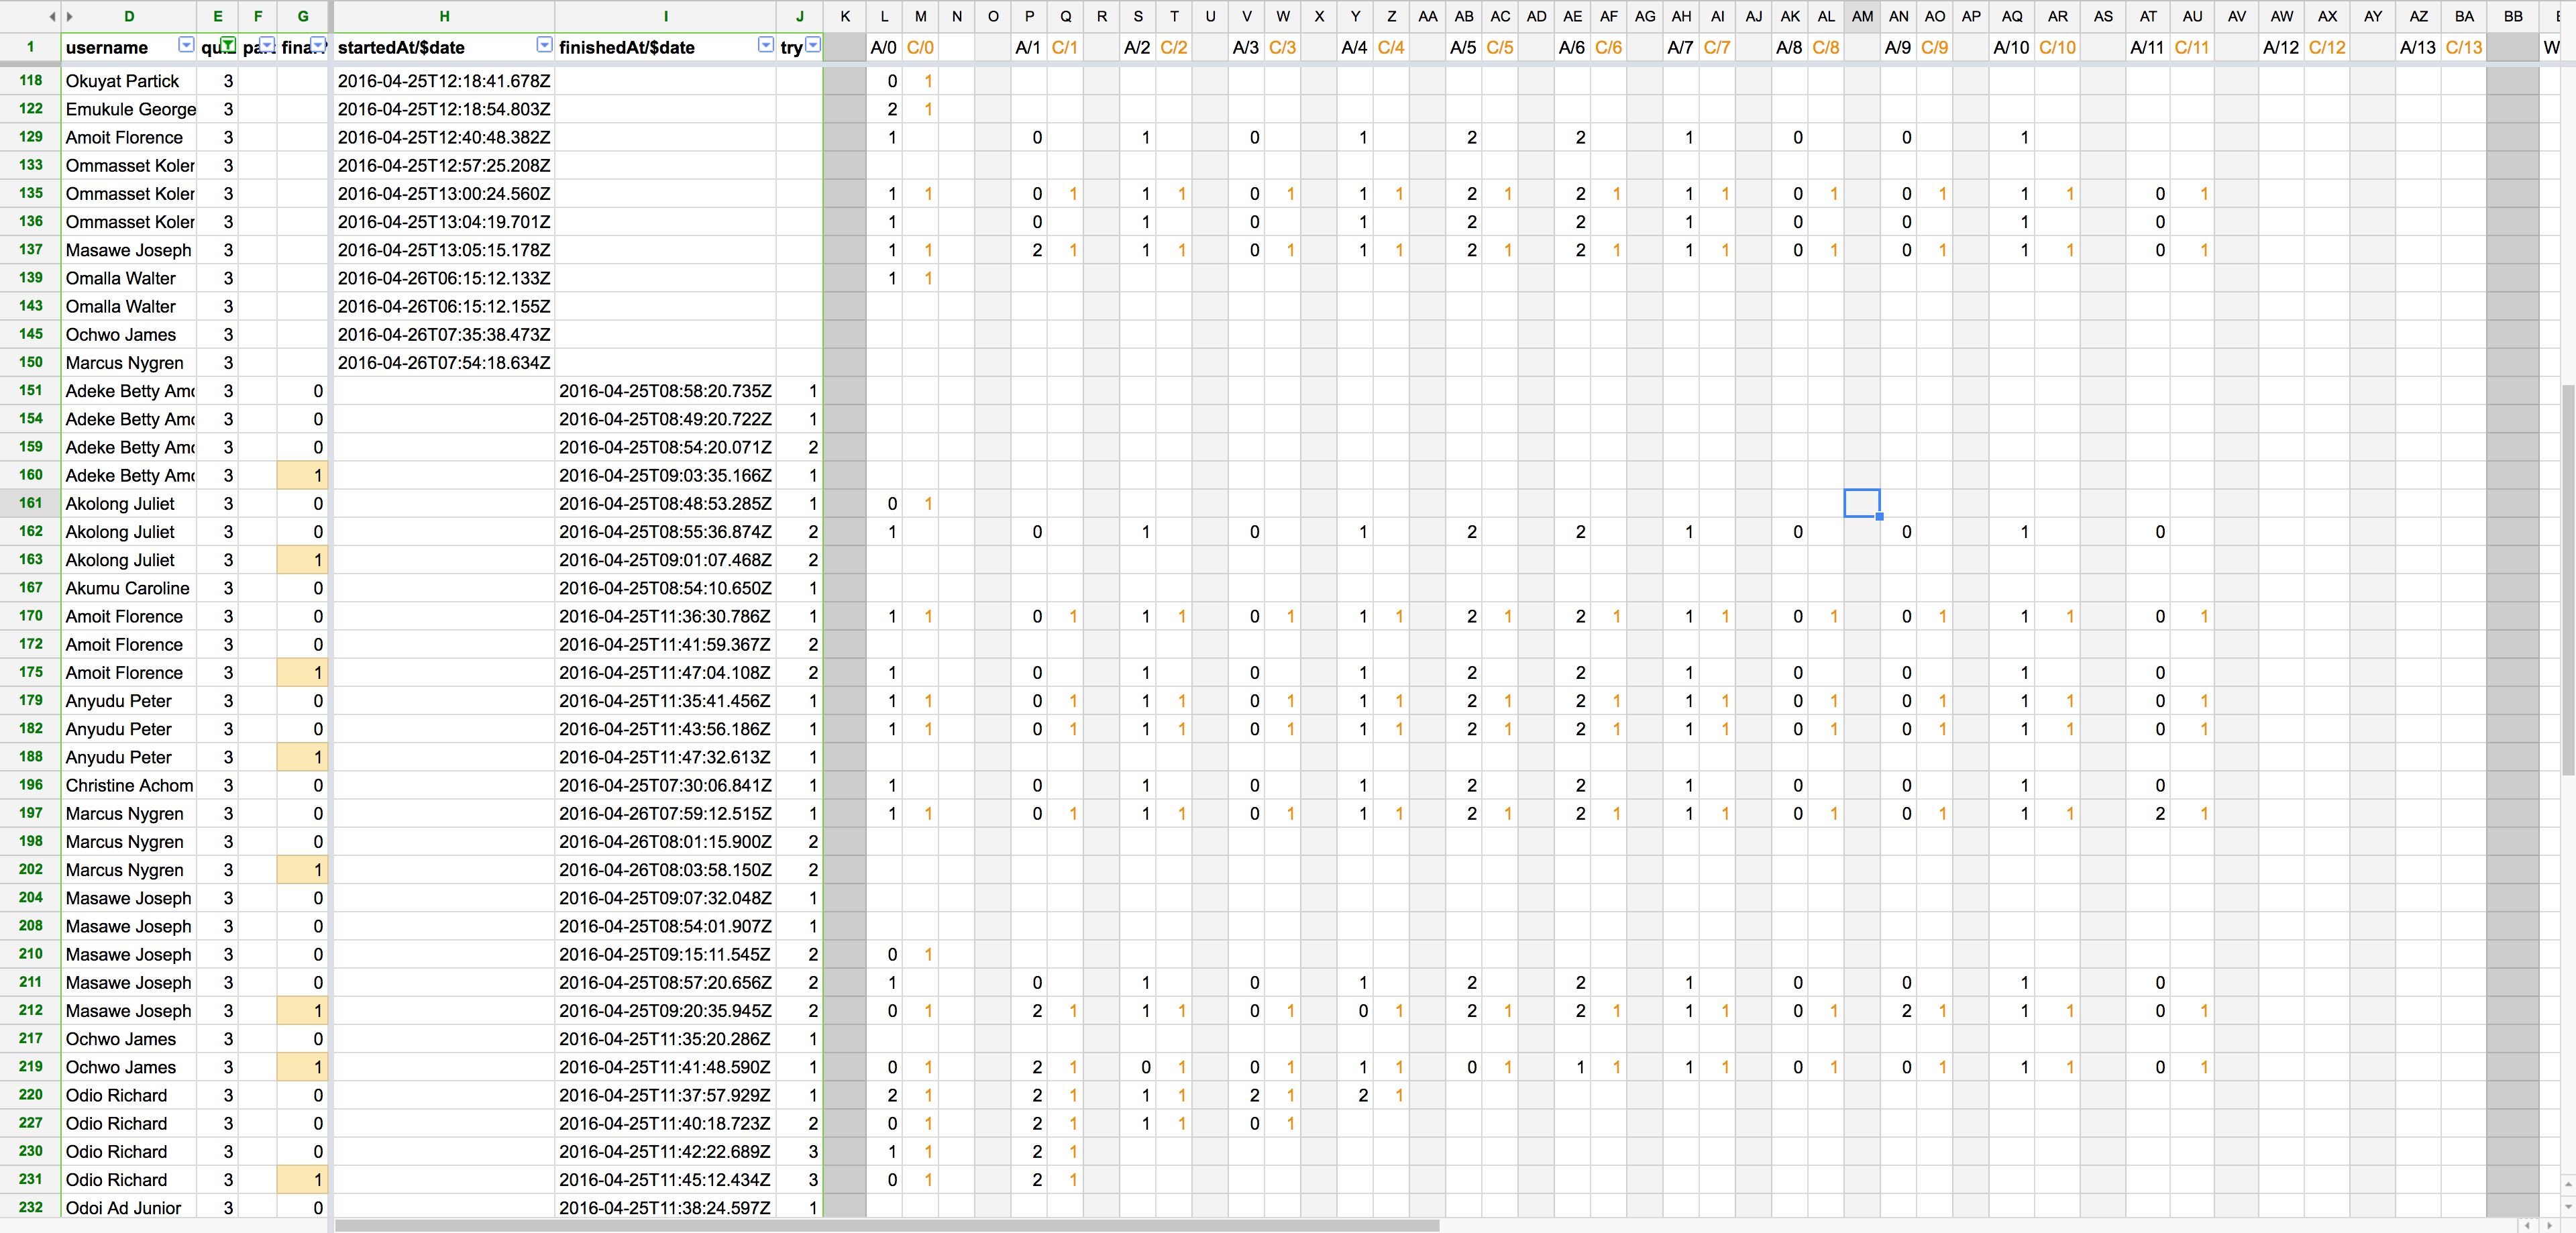
\includegraphics[width=0.9\textwidth]{analysis/resultsColored.png}
    \caption{The quiz results collected in a Google Sheet after data enhancement. In this figure, cell E1 has been filtered so that only results for quiz 3 are shown. Conditional formatting has been done with row G so that if it is a certification quiz, yellow color is used.}
    \label{fig:resultsColored}
\end{figure}

To be able to compare the test results with the pre-test results, it was clear that it would not be viable to test every dimension against every dimension. Instead, since goals of the app evaluation had been predefined in the following way, the quiz results were summarized into a new sheet so that the following could be derived:

\begin{itemize}
\item \% correct 1st try
\item number of tries until 100\%
\item number of tries until 100\% in 1 try
\end{itemize}

These could be calculated by having columns for:

\begin{itemize}
  \item Quiz 3
  \begin{itemize}
    \item Start time training
    \item \% correct 1st try
    \item number of tries until 100\% in 1 try
    \item Time difference start to end time certification
  \end{itemize}
  \item Quiz 9
  \begin{itemize}
    \item Start time training
    \item \% correct 1st try
    \item Time difference start to end 1st try
    \item Time difference start to passed training
    \item Time difference 1st try to certified
  \end{itemize}
\end{itemize}

Then, to see trends, color scales were again added. With ordinal values, a sequential color scheme is used (for example fastest time, from green to red), and with nominal values (like if they are female or male) where there is no right value, a qualitative color scheme is used. Now it was easier to spot outliers and trends, and giving validation to findings from notes and observations made during interviews, workshops and app tests.

\subsubsection{Step 4: Date Enhancement of Pre-study Results}
To see differences in answers more clearly, the data from the pre-study was made sortable and filterable. Then, the data was resampled for each column that had numerable (sortable) data in text instead of numbers, so for example "The day before" was changed to -1 and "The same day" to 0. In a similar way, school level was divided into four different groups, from 0 to 3, where 0 meant secondary, year unknown, 1 meant lower secondary, 2 meant upper secondary, and 3 meant tertiary.

After this, each column was given conditional formats using a color scale, using Google Sheets built-in functionality. This gave a visual way to quickly get an overview of the pre-test data.

\subsubsection{Step 5: Data Enhancement by Joining Pre-test and Results Summary}

The summary sheet and the pre-quiz sheet were joined, becoming a multiple-variate data set (several dimensions that were to bee compared with several other dimensions), see figure \ref{fig:analysFarg3}. A meeting with the university supervisors was held, so they could further give support in how to properly analyse the data. Since the two control groups showed similar means on the pre-quiz results, the two control groups were determined comparable.

\begin{figure}[h]
    \centering
    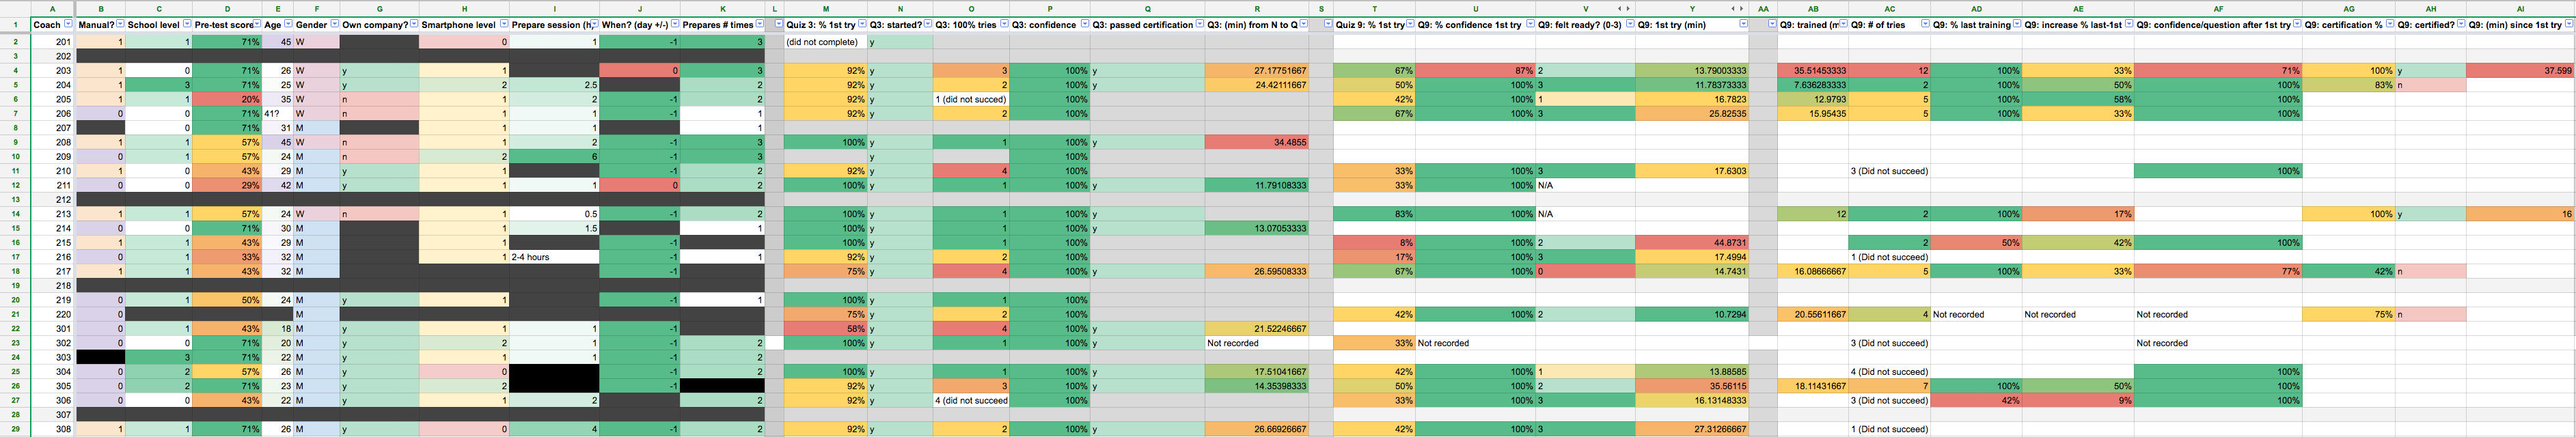
\includegraphics[width=1.0\textwidth]{analysis/sheets/0Overview.png}
    \caption{The multi-variate data set, made filterable and sortable in Google Sheets. Color scales and calculating means makes it easier to compare characteristics of the coach together with pre-test and quiz results. However, it is cumbersome and hard to quickly filter data on multiple parameters.}.
    \label{fig:analysFarg3}
\end{figure}

To meet the challenges of using Google Sheets, a multivariate analyzation software or a visualization was suggested to discover the data in less time. It was hard to determine a suitable multivariate analysis software suitable when having so few data points. Principle Component Analysis or Cohen's kappa would not be suitable, neither was it believed applicable to do Linear correlation on all dimensions. After discussion with other Master thesis students working with analysing data from various disciplines, parallel coordinates was suggested. It would allow very quickly filtering of the data, finding correlations, and distinguish outliers and common characteristics.

To guide the usage of the parallel coordinates (as there is so much to discover in the data set), using R to do Logistic correlation was also done. A disadvantage with this method, is that to be statistically significant, many data points may be needed, and it was now known before-hand if the method would be useful. Probably, parallel coordinates would be the best method to analyse a small multi-variate data set.

\subsubsection{Step 6: Visualization Mapping}
The goal with visualization mapping is to generate renderable data, in this case for the parallel coordinates visualization. Thus, a new spreadsheet is added, specific for visualizing the data. Columns were deleted that would serve no visual purpose (for example timestamps), gave all cells data values (even N/A when undefined), deleting users that did not have data, and shortened the column names so they would fit on the screen. The data was then exported from the Google Sheet into CSV.

\subsubsection{Step 7: Rendering}

For rendering, the JavaScript library D3.js, \citep{d3} was chosen. It supports data-driven documents for visualizing data with HTML, SVG and CSS. It supports both JSON and CSV data. A visual framework for multidimensional detectives for D3.js was found called "Parcoords.js", \cite{parcoords}. The example code from "Linking with a Data Table" provided the basis for the rendering. It allowed observing both the parallel coordinates visualization and the table data from the Google Sheet simultaneously.
% https://syntagmatic.github.io/parallel-coordinates/
% Chang, K. (2012). Parallel Coordinates toolkit : Parcoords.js 0.1. Parallel Coordinates toolkit. Retrieved September 8, 2012, from http://syntagmatic.github.com/parallel-coordinates/
% Kosara, R. (2010, May 13). Parallel Coordinates. Eagereyes.org. Retrieved September 8, 2012, from http://eagereyes.org/techniques/parallel-coordinates
% Tricaud, S. (2008). Picviz: finding a needle in a haystack. Proceedings WASL, San Diego. Retrieved from http://www.usenix.org/events/wasl08/tech/full_papers/tricaud/tricaud.pdf

 %https://syntagmatic.github.io/parallel-coordinates/examples/table.html

To work, the example CSV file was replaced with the data from exporting the Google Sheets data. To benefit the visualization, also the colors were changed, and the toolkit's functionality to drag the axes titles around to reorder the dimensions was used, since the goal was to quickly compare and find correlations. The result is visible in \ref{fig:parallell-coordinates-1}.

\begin{figure}[h]
    \centering
    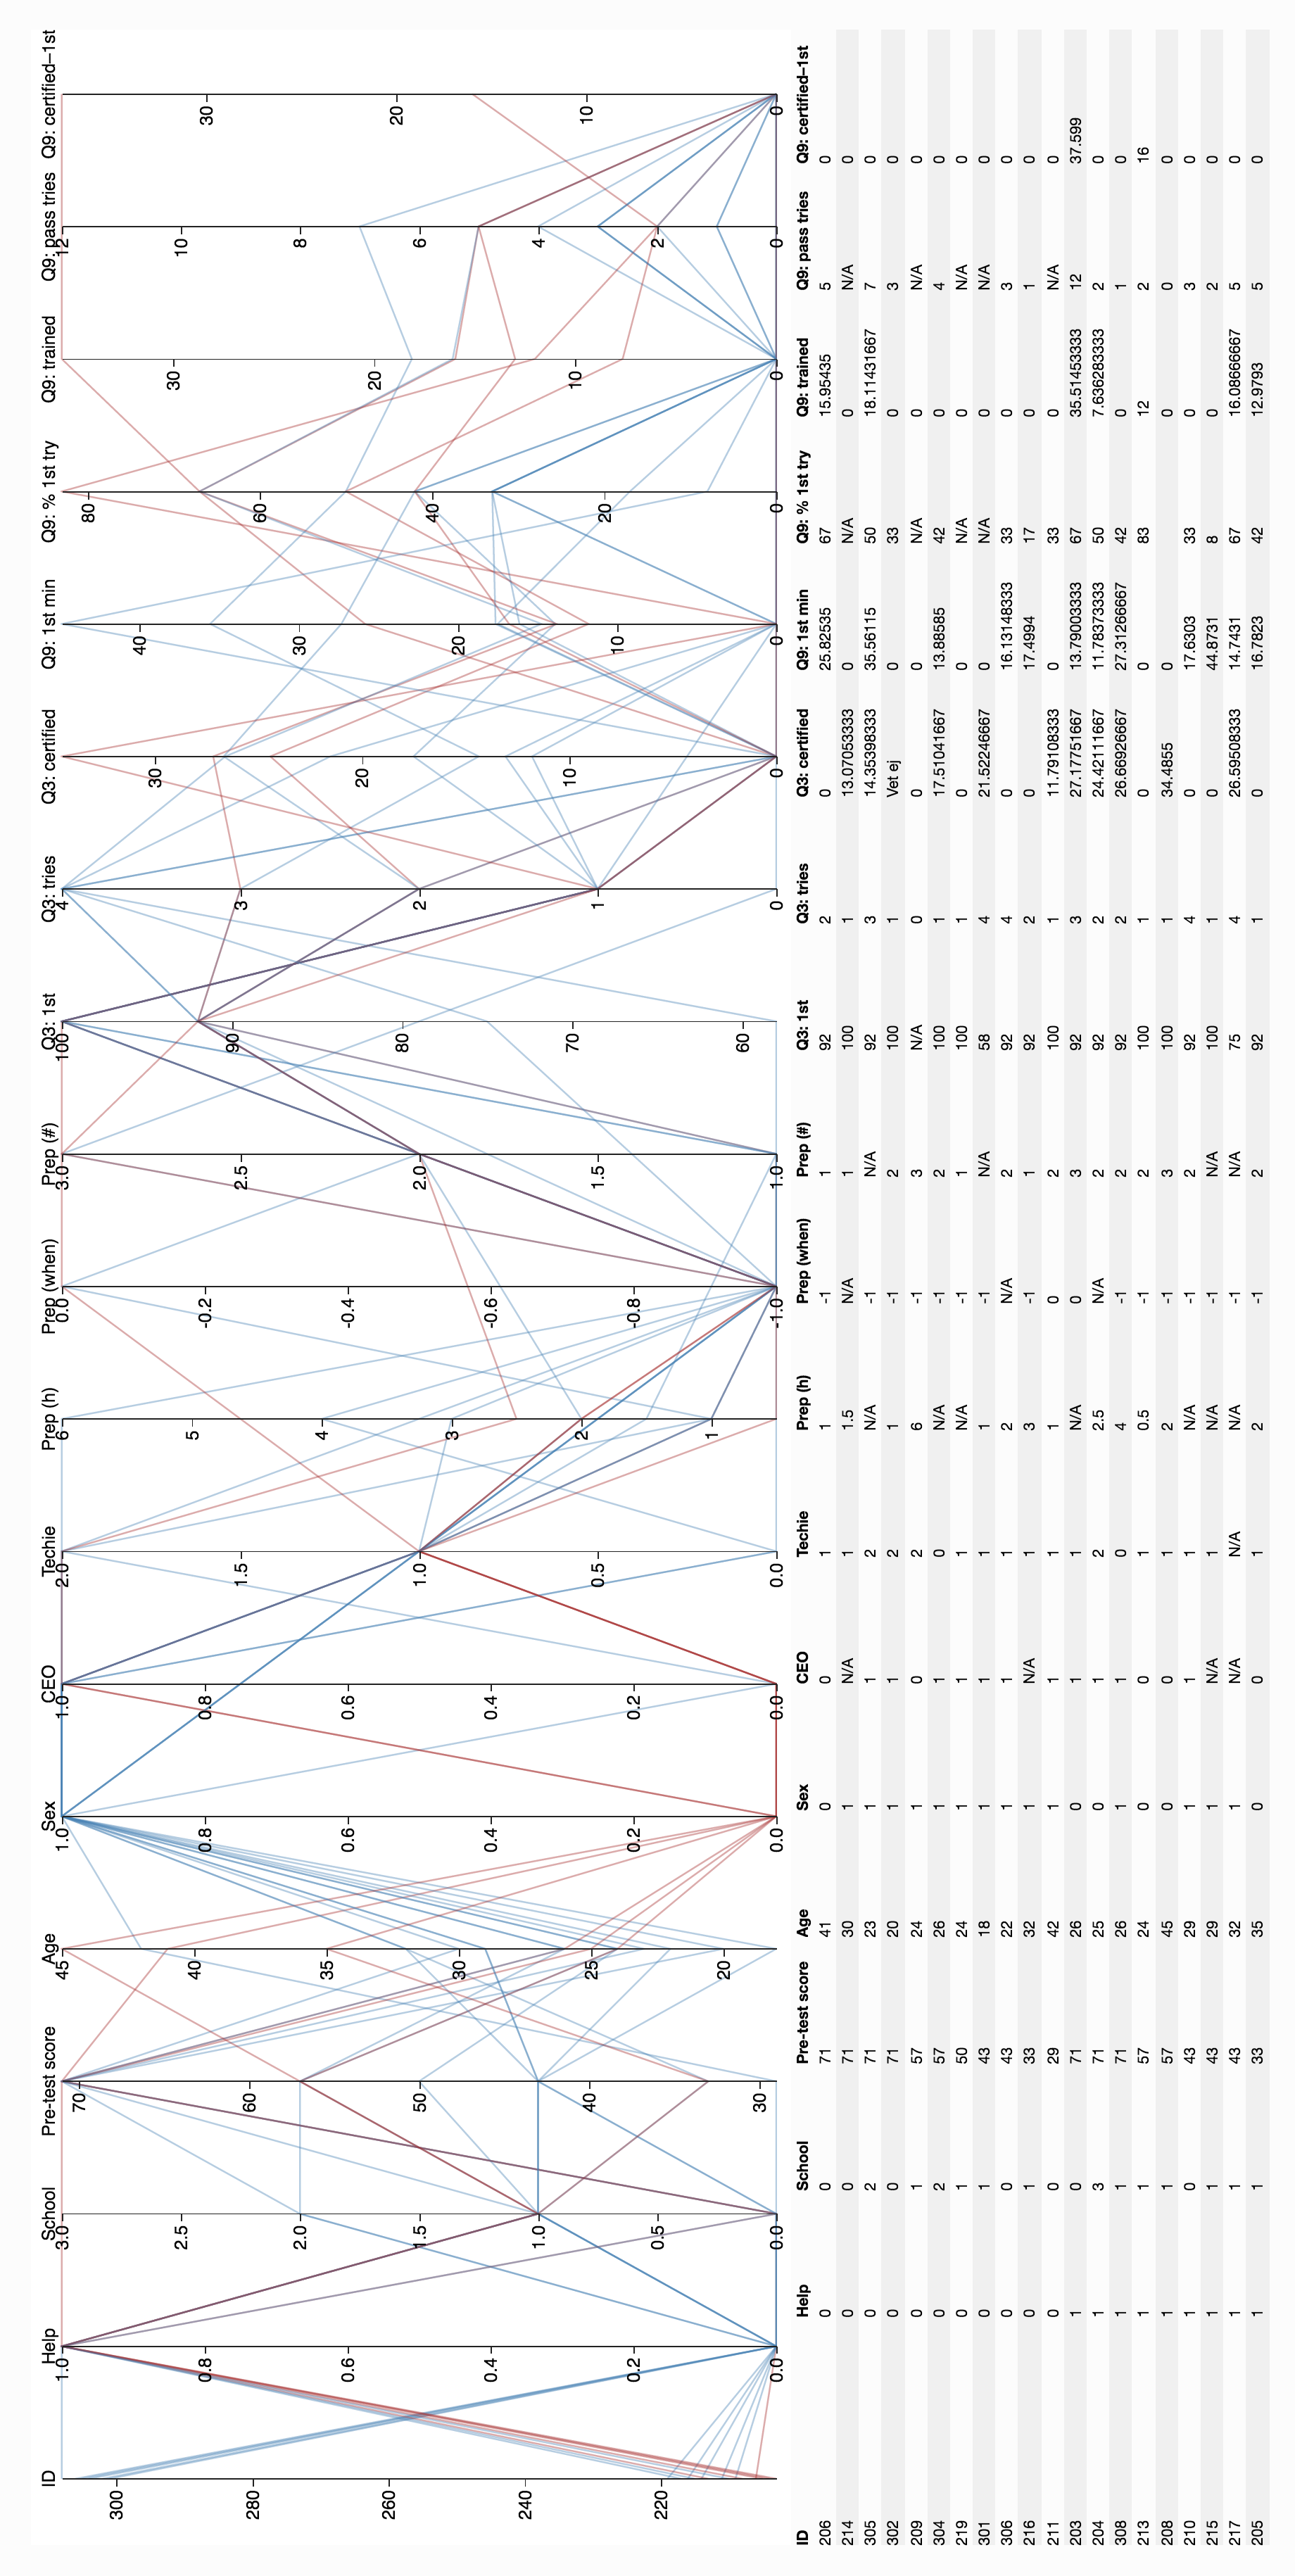
\includegraphics[width=0.7\textwidth]{analysis/parallellCoordinates3.png}
    \caption{The parallel coordinates visualization, done in d3.js. The visualization support draggable axes, filtering of data via dragging the sliders (which synchronizes with the data table), color assignment (like blue and red for men and women in the example), and hovering over a specific data point.}
    \label{fig:parallell-coordinates-1}
\end{figure}


